\documentclass[11pt]{article}
\usepackage[english]{babel}
\usepackage[utf8x]{inputenc}
\usepackage[table]{xcolor}
\usepackage{amsmath}
\usepackage{graphicx}
\graphicspath{{Images/}}
\usepackage{hyperref}
\usepackage{float}
\usepackage{todonotes}
\usepackage[linesnumbered,algoruled,boxed,lined]{algorithm2e}
\usepackage[a4paper, margin=2.5cm]{geometry}
\usepackage{geometry}
\usepackage[title,toc,page]{appendix}
% \usepackage{fullpage}
\usepackage{fancyhdr}
%\pagestyle{fancy}
\usepackage{listings}
\usepackage{pgfplots} 


\usepackage{caption}
\usepackage{subcaption}

%%%%%%%%%%%%%%%%%%%%%%%%%%%%
%For jupyter notebook stylings
%%%%%%%%%%%%%%%%%%%%%%%%%%%%%
%For jupyter notebook stylings
%%%%%%%%%%%%%%%%%%%%%%%%%%%%%
%For jupyter notebook stylings
%\include{incl_packages.tex}

\usepackage[breakable]{tcolorbox}
\tcbset{nobeforeafter} % prevents tcolorboxes being placing in paragraphs
\usepackage{float}
\floatplacement{figure}{H} % forces figures to be placed at the correct location

\usepackage[T1]{fontenc}
% Nicer default font (+ math font) than Computer Modern for most use cases
\usepackage{mathpazo}

% Exact colors from NB
\definecolor{incolor}{HTML}{303F9F}
\definecolor{outcolor}{HTML}{D84315}
\definecolor{cellborder}{HTML}{CFCFCF}
\definecolor{cellbackground}{HTML}{F7F7F7}

% prompt
\newcommand{\prompt}[4]{
    \llap{{\color{#2}[#3]: #4}}\vspace{-1.25em}
}


\usepackage{upquote} % Upright quotes for verbatim code
\usepackage{eurosym} % defines \euro
%\usepackage[mathletters]{ucs} % Extended unicode (utf-8) support
\usepackage[utf8x]{inputenc} % Allow utf-8 characters in the tex document
\usepackage{fancyvrb} % verbatim replacement that allows latex
\usepackage{grffile} % extends the file name processing of package graphics 
                     % to support a larger range 
% The hyperref package gives us a pdf with properly built
% internal navigation ('pdf bookmarks' for the table of contents,
% internal cross-reference links, web links for URLs, etc.)
\usepackage{hyperref}
\usepackage{longtable} % longtable support required by pandoc >1.10
\usepackage{booktabs}  % table support for pandoc > 1.12.2
\usepackage[inline]{enumitem} % IRkernel/repr support (it uses the enumerate* environment)
\usepackage[normalem]{ulem} % ulem is needed to support strikethroughs (\sout)
                            % normalem makes italics be italics, not underlines
\usepackage{mathrsfs}


    
    % Pygments definitions
\makeatletter
\def\PY@reset{\let\PY@it=\relax \let\PY@bf=\relax%
    \let\PY@ul=\relax \let\PY@tc=\relax%
    \let\PY@bc=\relax \let\PY@ff=\relax}
\def\PY@tok#1{\csname PY@tok@#1\endcsname}
\def\PY@toks#1+{\ifx\relax#1\empty\else%
    \PY@tok{#1}\expandafter\PY@toks\fi}
\def\PY@do#1{\PY@bc{\PY@tc{\PY@ul{%
    \PY@it{\PY@bf{\PY@ff{#1}}}}}}}
\def\PY#1#2{\PY@reset\PY@toks#1+\relax+\PY@do{#2}}
    
    
\expandafter\def\csname PY@tok@w\endcsname{\def\PY@tc##1{\textcolor[rgb]{0.73,0.73,0.73}{##1}}}
\expandafter\def\csname PY@tok@c\endcsname{\let\PY@it=\textit\def\PY@tc##1{\textcolor[rgb]{0.25,0.50,0.50}{##1}}}
\expandafter\def\csname PY@tok@cp\endcsname{\def\PY@tc##1{\textcolor[rgb]{0.74,0.48,0.00}{##1}}}
\expandafter\def\csname PY@tok@k\endcsname{\let\PY@bf=\textbf\def\PY@tc##1{\textcolor[rgb]{0.00,0.50,0.00}{##1}}}
\expandafter\def\csname PY@tok@kp\endcsname{\def\PY@tc##1{\textcolor[rgb]{0.00,0.50,0.00}{##1}}}
\expandafter\def\csname PY@tok@kt\endcsname{\def\PY@tc##1{\textcolor[rgb]{0.69,0.00,0.25}{##1}}}
\expandafter\def\csname PY@tok@o\endcsname{\def\PY@tc##1{\textcolor[rgb]{0.40,0.40,0.40}{##1}}}
\expandafter\def\csname PY@tok@ow\endcsname{\let\PY@bf=\textbf\def\PY@tc##1{\textcolor[rgb]{0.67,0.13,1.00}{##1}}}
\expandafter\def\csname PY@tok@nb\endcsname{\def\PY@tc##1{\textcolor[rgb]{0.00,0.50,0.00}{##1}}}
\expandafter\def\csname PY@tok@nf\endcsname{\def\PY@tc##1{\textcolor[rgb]{0.00,0.00,1.00}{##1}}}
\expandafter\def\csname PY@tok@nc\endcsname{\let\PY@bf=\textbf\def\PY@tc##1{\textcolor[rgb]{0.00,0.00,1.00}{##1}}}
\expandafter\def\csname PY@tok@nn\endcsname{\let\PY@bf=\textbf\def\PY@tc##1{\textcolor[rgb]{0.00,0.00,1.00}{##1}}}
\expandafter\def\csname PY@tok@ne\endcsname{\let\PY@bf=\textbf\def\PY@tc##1{\textcolor[rgb]{0.82,0.25,0.23}{##1}}}
\expandafter\def\csname PY@tok@nv\endcsname{\def\PY@tc##1{\textcolor[rgb]{0.10,0.09,0.49}{##1}}}
\expandafter\def\csname PY@tok@no\endcsname{\def\PY@tc##1{\textcolor[rgb]{0.53,0.00,0.00}{##1}}}
\expandafter\def\csname PY@tok@nl\endcsname{\def\PY@tc##1{\textcolor[rgb]{0.63,0.63,0.00}{##1}}}
\expandafter\def\csname PY@tok@ni\endcsname{\let\PY@bf=\textbf\def\PY@tc##1{\textcolor[rgb]{0.60,0.60,0.60}{##1}}}
\expandafter\def\csname PY@tok@na\endcsname{\def\PY@tc##1{\textcolor[rgb]{0.49,0.56,0.16}{##1}}}
\expandafter\def\csname PY@tok@nt\endcsname{\let\PY@bf=\textbf\def\PY@tc##1{\textcolor[rgb]{0.00,0.50,0.00}{##1}}}
\expandafter\def\csname PY@tok@nd\endcsname{\def\PY@tc##1{\textcolor[rgb]{0.67,0.13,1.00}{##1}}}
\expandafter\def\csname PY@tok@s\endcsname{\def\PY@tc##1{\textcolor[rgb]{0.73,0.13,0.13}{##1}}}
\expandafter\def\csname PY@tok@sd\endcsname{\let\PY@it=\textit\def\PY@tc##1{\textcolor[rgb]{0.73,0.13,0.13}{##1}}}
\expandafter\def\csname PY@tok@si\endcsname{\let\PY@bf=\textbf\def\PY@tc##1{\textcolor[rgb]{0.73,0.40,0.53}{##1}}}
\expandafter\def\csname PY@tok@se\endcsname{\let\PY@bf=\textbf\def\PY@tc##1{\textcolor[rgb]{0.73,0.40,0.13}{##1}}}
\expandafter\def\csname PY@tok@sr\endcsname{\def\PY@tc##1{\textcolor[rgb]{0.73,0.40,0.53}{##1}}}
\expandafter\def\csname PY@tok@ss\endcsname{\def\PY@tc##1{\textcolor[rgb]{0.10,0.09,0.49}{##1}}}
\expandafter\def\csname PY@tok@sx\endcsname{\def\PY@tc##1{\textcolor[rgb]{0.00,0.50,0.00}{##1}}}
\expandafter\def\csname PY@tok@m\endcsname{\def\PY@tc##1{\textcolor[rgb]{0.40,0.40,0.40}{##1}}}
\expandafter\def\csname PY@tok@gh\endcsname{\let\PY@bf=\textbf\def\PY@tc##1{\textcolor[rgb]{0.00,0.00,0.50}{##1}}}
\expandafter\def\csname PY@tok@gu\endcsname{\let\PY@bf=\textbf\def\PY@tc##1{\textcolor[rgb]{0.50,0.00,0.50}{##1}}}
\expandafter\def\csname PY@tok@gd\endcsname{\def\PY@tc##1{\textcolor[rgb]{0.63,0.00,0.00}{##1}}}
\expandafter\def\csname PY@tok@gi\endcsname{\def\PY@tc##1{\textcolor[rgb]{0.00,0.63,0.00}{##1}}}
\expandafter\def\csname PY@tok@gr\endcsname{\def\PY@tc##1{\textcolor[rgb]{1.00,0.00,0.00}{##1}}}
\expandafter\def\csname PY@tok@ge\endcsname{\let\PY@it=\textit}
\expandafter\def\csname PY@tok@gs\endcsname{\let\PY@bf=\textbf}
\expandafter\def\csname PY@tok@gp\endcsname{\let\PY@bf=\textbf\def\PY@tc##1{\textcolor[rgb]{0.00,0.00,0.50}{##1}}}
\expandafter\def\csname PY@tok@go\endcsname{\def\PY@tc##1{\textcolor[rgb]{0.53,0.53,0.53}{##1}}}
\expandafter\def\csname PY@tok@gt\endcsname{\def\PY@tc##1{\textcolor[rgb]{0.00,0.27,0.87}{##1}}}
\expandafter\def\csname PY@tok@err\endcsname{\def\PY@bc##1{\setlength{\fboxsep}{0pt}\fcolorbox[rgb]{1.00,0.00,0.00}{1,1,1}{\strut ##1}}}
\expandafter\def\csname PY@tok@kc\endcsname{\let\PY@bf=\textbf\def\PY@tc##1{\textcolor[rgb]{0.00,0.50,0.00}{##1}}}
\expandafter\def\csname PY@tok@kd\endcsname{\let\PY@bf=\textbf\def\PY@tc##1{\textcolor[rgb]{0.00,0.50,0.00}{##1}}}
\expandafter\def\csname PY@tok@kn\endcsname{\let\PY@bf=\textbf\def\PY@tc##1{\textcolor[rgb]{0.00,0.50,0.00}{##1}}}
\expandafter\def\csname PY@tok@kr\endcsname{\let\PY@bf=\textbf\def\PY@tc##1{\textcolor[rgb]{0.00,0.50,0.00}{##1}}}
\expandafter\def\csname PY@tok@bp\endcsname{\def\PY@tc##1{\textcolor[rgb]{0.00,0.50,0.00}{##1}}}
\expandafter\def\csname PY@tok@fm\endcsname{\def\PY@tc##1{\textcolor[rgb]{0.00,0.00,1.00}{##1}}}
\expandafter\def\csname PY@tok@vc\endcsname{\def\PY@tc##1{\textcolor[rgb]{0.10,0.09,0.49}{##1}}}
\expandafter\def\csname PY@tok@vg\endcsname{\def\PY@tc##1{\textcolor[rgb]{0.10,0.09,0.49}{##1}}}
\expandafter\def\csname PY@tok@vi\endcsname{\def\PY@tc##1{\textcolor[rgb]{0.10,0.09,0.49}{##1}}}
\expandafter\def\csname PY@tok@vm\endcsname{\def\PY@tc##1{\textcolor[rgb]{0.10,0.09,0.49}{##1}}}
\expandafter\def\csname PY@tok@sa\endcsname{\def\PY@tc##1{\textcolor[rgb]{0.73,0.13,0.13}{##1}}}
\expandafter\def\csname PY@tok@sb\endcsname{\def\PY@tc##1{\textcolor[rgb]{0.73,0.13,0.13}{##1}}}
\expandafter\def\csname PY@tok@sc\endcsname{\def\PY@tc##1{\textcolor[rgb]{0.73,0.13,0.13}{##1}}}
\expandafter\def\csname PY@tok@dl\endcsname{\def\PY@tc##1{\textcolor[rgb]{0.73,0.13,0.13}{##1}}}
\expandafter\def\csname PY@tok@s2\endcsname{\def\PY@tc##1{\textcolor[rgb]{0.73,0.13,0.13}{##1}}}
\expandafter\def\csname PY@tok@sh\endcsname{\def\PY@tc##1{\textcolor[rgb]{0.73,0.13,0.13}{##1}}}
\expandafter\def\csname PY@tok@s1\endcsname{\def\PY@tc##1{\textcolor[rgb]{0.73,0.13,0.13}{##1}}}
\expandafter\def\csname PY@tok@mb\endcsname{\def\PY@tc##1{\textcolor[rgb]{0.40,0.40,0.40}{##1}}}
\expandafter\def\csname PY@tok@mf\endcsname{\def\PY@tc##1{\textcolor[rgb]{0.40,0.40,0.40}{##1}}}
\expandafter\def\csname PY@tok@mh\endcsname{\def\PY@tc##1{\textcolor[rgb]{0.40,0.40,0.40}{##1}}}
\expandafter\def\csname PY@tok@mi\endcsname{\def\PY@tc##1{\textcolor[rgb]{0.40,0.40,0.40}{##1}}}
\expandafter\def\csname PY@tok@il\endcsname{\def\PY@tc##1{\textcolor[rgb]{0.40,0.40,0.40}{##1}}}
\expandafter\def\csname PY@tok@mo\endcsname{\def\PY@tc##1{\textcolor[rgb]{0.40,0.40,0.40}{##1}}}
\expandafter\def\csname PY@tok@ch\endcsname{\let\PY@it=\textit\def\PY@tc##1{\textcolor[rgb]{0.25,0.50,0.50}{##1}}}
\expandafter\def\csname PY@tok@cm\endcsname{\let\PY@it=\textit\def\PY@tc##1{\textcolor[rgb]{0.25,0.50,0.50}{##1}}}
\expandafter\def\csname PY@tok@cpf\endcsname{\let\PY@it=\textit\def\PY@tc##1{\textcolor[rgb]{0.25,0.50,0.50}{##1}}}
\expandafter\def\csname PY@tok@c1\endcsname{\let\PY@it=\textit\def\PY@tc##1{\textcolor[rgb]{0.25,0.50,0.50}{##1}}}
\expandafter\def\csname PY@tok@cs\endcsname{\let\PY@it=\textit\def\PY@tc##1{\textcolor[rgb]{0.25,0.50,0.50}{##1}}}

\def\PYZbs{\char`\\}
\def\PYZus{\char`\_}
\def\PYZob{\char`\{}
\def\PYZcb{\char`\}}
\def\PYZca{\char`\^}
\def\PYZam{\char`\&}
\def\PYZlt{\char`\<}
\def\PYZgt{\char`\>}
\def\PYZsh{\char`\#}
\def\PYZpc{\char`\%}
\def\PYZdl{\char`\$}
\def\PYZhy{\char`\-}
\def\PYZsq{\char`\'}
\def\PYZdq{\char`\"}
\def\PYZti{\char`\~}
    
    
    % For linebreaks inside Verbatim environment from package fancyvrb. 
    \makeatletter
        \newbox\Wrappedcontinuationbox 
        \newbox\Wrappedvisiblespacebox 
        \newcommand*\Wrappedvisiblespace {\textcolor{red}{\textvisiblespace}} 
        \newcommand*\Wrappedcontinuationsymbol {\textcolor{red}{\llap{\tiny$\m@th\hookrightarrow$}}} 
        \newcommand*\Wrappedcontinuationindent {3ex } 
        \newcommand*\Wrappedafterbreak {\kern\Wrappedcontinuationindent\copy\Wrappedcontinuationbox} 
        % Take advantage of the already applied Pygments mark-up to insert 
        % potential linebreaks for TeX processing. 
        %        {, <, #, %, $, ' and ": go to next line. 
        %        _, }, ^, &, >, - and ~: stay at end of broken line. 
        % Use of \textquotesingle for straight quote. 
        \newcommand*\Wrappedbreaksatspecials {% 
            \def\PYGZus{\discretionary{\char`\_}{\Wrappedafterbreak}{\char`\_}}% 
            \def\PYGZob{\discretionary{}{\Wrappedafterbreak\char`\{}{\char`\{}}% 
            \def\PYGZcb{\discretionary{\char`\}}{\Wrappedafterbreak}{\char`\}}}% 
            \def\PYGZca{\discretionary{\char`\^}{\Wrappedafterbreak}{\char`\^}}% 
            \def\PYGZam{\discretionary{\char`\&}{\Wrappedafterbreak}{\char`\&}}% 
            \def\PYGZlt{\discretionary{}{\Wrappedafterbreak\char`\<}{\char`\<}}% 
            \def\PYGZgt{\discretionary{\char`\>}{\Wrappedafterbreak}{\char`\>}}% 
            \def\PYGZsh{\discretionary{}{\Wrappedafterbreak\char`\#}{\char`\#}}% 
            \def\PYGZpc{\discretionary{}{\Wrappedafterbreak\char`\%}{\char`\%}}% 
            \def\PYGZdl{\discretionary{}{\Wrappedafterbreak\char`\$}{\char`\$}}% 
            \def\PYGZhy{\discretionary{\char`\-}{\Wrappedafterbreak}{\char`\-}}% 
            \def\PYGZsq{\discretionary{}{\Wrappedafterbreak\textquotesingle}{\textquotesingle}}% 
            \def\PYGZdq{\discretionary{}{\Wrappedafterbreak\char`\"}{\char`\"}}% 
            \def\PYGZti{\discretionary{\char`\~}{\Wrappedafterbreak}{\char`\~}}% 
        } 
        % Some characters . , ; ? ! / are not pygmentized. 
        % This macro makes them "active" and they will insert potential linebreaks 
        \newcommand*\Wrappedbreaksatpunct {% 
            \lccode`\~`\.\lowercase{\def~}{\discretionary{\hbox{\char`\.}}{\Wrappedafterbreak}{\hbox{\char`\.}}}% 
            \lccode`\~`\,\lowercase{\def~}{\discretionary{\hbox{\char`\,}}{\Wrappedafterbreak}{\hbox{\char`\,}}}% 
            \lccode`\~`\;\lowercase{\def~}{\discretionary{\hbox{\char`\;}}{\Wrappedafterbreak}{\hbox{\char`\;}}}% 
            \lccode`\~`\:\lowercase{\def~}{\discretionary{\hbox{\char`\:}}{\Wrappedafterbreak}{\hbox{\char`\:}}}% 
            \lccode`\~`\?\lowercase{\def~}{\discretionary{\hbox{\char`\?}}{\Wrappedafterbreak}{\hbox{\char`\?}}}% 
            \lccode`\~`\!\lowercase{\def~}{\discretionary{\hbox{\char`\!}}{\Wrappedafterbreak}{\hbox{\char`\!}}}% 
            \lccode`\~`\/\lowercase{\def~}{\discretionary{\hbox{\char`\/}}{\Wrappedafterbreak}{\hbox{\char`\/}}}% 
            \catcode`\.\active
            \catcode`\,\active 
            \catcode`\;\active
            \catcode`\:\active
            \catcode`\?\active
            \catcode`\!\active
            \catcode`\/\active 
            \lccode`\~`\~ 	
        }
    \makeatother

    \let\OriginalVerbatim=\Verbatim
    \makeatletter
    \renewcommand{\Verbatim}[1][1]{%
        %\parskip\z@skip
        \sbox\Wrappedcontinuationbox {\Wrappedcontinuationsymbol}%
        \sbox\Wrappedvisiblespacebox {\FV@SetupFont\Wrappedvisiblespace}%
        \def\FancyVerbFormatLine ##1{\hsize\linewidth
            \vtop{\raggedright\hyphenpenalty\z@\exhyphenpenalty\z@
                \doublehyphendemerits\z@\finalhyphendemerits\z@
                \strut ##1\strut}%
        }%
        % If the linebreak is at a space, the latter will be displayed as visible
        % space at end of first line, and a continuation symbol starts next line.
        % Stretch/shrink are however usually zero for typewriter font.
        \def\FV@Space {%
            \nobreak\hskip\z@ plus\fontdimen3\font minus\fontdimen4\font
            \discretionary{\copy\Wrappedvisiblespacebox}{\Wrappedafterbreak}
            {\kern\fontdimen2\font}%
        }%
        
        % Allow breaks at special characters using \PYG... macros.
        \Wrappedbreaksatspecials
        % Breaks at punctuation characters . , ; ? ! and / need catcode=\active 	
        \OriginalVerbatim[#1,codes*=\Wrappedbreaksatpunct]%
    }
    \makeatother

\usepackage[breakable]{tcolorbox}
\tcbset{nobeforeafter} % prevents tcolorboxes being placing in paragraphs
\usepackage{float}
\floatplacement{figure}{H} % forces figures to be placed at the correct location

\usepackage[T1]{fontenc}
% Nicer default font (+ math font) than Computer Modern for most use cases
\usepackage{mathpazo}

% Exact colors from NB
\definecolor{incolor}{HTML}{303F9F}
\definecolor{outcolor}{HTML}{D84315}
\definecolor{cellborder}{HTML}{CFCFCF}
\definecolor{cellbackground}{HTML}{F7F7F7}

% prompt
\newcommand{\prompt}[4]{
    \llap{{\color{#2}[#3]: #4}}\vspace{-1.25em}
}


\usepackage{upquote} % Upright quotes for verbatim code
\usepackage{eurosym} % defines \euro
%\usepackage[mathletters]{ucs} % Extended unicode (utf-8) support
\usepackage[utf8x]{inputenc} % Allow utf-8 characters in the tex document
\usepackage{fancyvrb} % verbatim replacement that allows latex
\usepackage{grffile} % extends the file name processing of package graphics 
                     % to support a larger range 
% The hyperref package gives us a pdf with properly built
% internal navigation ('pdf bookmarks' for the table of contents,
% internal cross-reference links, web links for URLs, etc.)
\usepackage{hyperref}
\usepackage{longtable} % longtable support required by pandoc >1.10
\usepackage{booktabs}  % table support for pandoc > 1.12.2
\usepackage[inline]{enumitem} % IRkernel/repr support (it uses the enumerate* environment)
\usepackage[normalem]{ulem} % ulem is needed to support strikethroughs (\sout)
                            % normalem makes italics be italics, not underlines
\usepackage{mathrsfs}


    
    % Pygments definitions
\makeatletter
\def\PY@reset{\let\PY@it=\relax \let\PY@bf=\relax%
    \let\PY@ul=\relax \let\PY@tc=\relax%
    \let\PY@bc=\relax \let\PY@ff=\relax}
\def\PY@tok#1{\csname PY@tok@#1\endcsname}
\def\PY@toks#1+{\ifx\relax#1\empty\else%
    \PY@tok{#1}\expandafter\PY@toks\fi}
\def\PY@do#1{\PY@bc{\PY@tc{\PY@ul{%
    \PY@it{\PY@bf{\PY@ff{#1}}}}}}}
\def\PY#1#2{\PY@reset\PY@toks#1+\relax+\PY@do{#2}}
    
    
\expandafter\def\csname PY@tok@w\endcsname{\def\PY@tc##1{\textcolor[rgb]{0.73,0.73,0.73}{##1}}}
\expandafter\def\csname PY@tok@c\endcsname{\let\PY@it=\textit\def\PY@tc##1{\textcolor[rgb]{0.25,0.50,0.50}{##1}}}
\expandafter\def\csname PY@tok@cp\endcsname{\def\PY@tc##1{\textcolor[rgb]{0.74,0.48,0.00}{##1}}}
\expandafter\def\csname PY@tok@k\endcsname{\let\PY@bf=\textbf\def\PY@tc##1{\textcolor[rgb]{0.00,0.50,0.00}{##1}}}
\expandafter\def\csname PY@tok@kp\endcsname{\def\PY@tc##1{\textcolor[rgb]{0.00,0.50,0.00}{##1}}}
\expandafter\def\csname PY@tok@kt\endcsname{\def\PY@tc##1{\textcolor[rgb]{0.69,0.00,0.25}{##1}}}
\expandafter\def\csname PY@tok@o\endcsname{\def\PY@tc##1{\textcolor[rgb]{0.40,0.40,0.40}{##1}}}
\expandafter\def\csname PY@tok@ow\endcsname{\let\PY@bf=\textbf\def\PY@tc##1{\textcolor[rgb]{0.67,0.13,1.00}{##1}}}
\expandafter\def\csname PY@tok@nb\endcsname{\def\PY@tc##1{\textcolor[rgb]{0.00,0.50,0.00}{##1}}}
\expandafter\def\csname PY@tok@nf\endcsname{\def\PY@tc##1{\textcolor[rgb]{0.00,0.00,1.00}{##1}}}
\expandafter\def\csname PY@tok@nc\endcsname{\let\PY@bf=\textbf\def\PY@tc##1{\textcolor[rgb]{0.00,0.00,1.00}{##1}}}
\expandafter\def\csname PY@tok@nn\endcsname{\let\PY@bf=\textbf\def\PY@tc##1{\textcolor[rgb]{0.00,0.00,1.00}{##1}}}
\expandafter\def\csname PY@tok@ne\endcsname{\let\PY@bf=\textbf\def\PY@tc##1{\textcolor[rgb]{0.82,0.25,0.23}{##1}}}
\expandafter\def\csname PY@tok@nv\endcsname{\def\PY@tc##1{\textcolor[rgb]{0.10,0.09,0.49}{##1}}}
\expandafter\def\csname PY@tok@no\endcsname{\def\PY@tc##1{\textcolor[rgb]{0.53,0.00,0.00}{##1}}}
\expandafter\def\csname PY@tok@nl\endcsname{\def\PY@tc##1{\textcolor[rgb]{0.63,0.63,0.00}{##1}}}
\expandafter\def\csname PY@tok@ni\endcsname{\let\PY@bf=\textbf\def\PY@tc##1{\textcolor[rgb]{0.60,0.60,0.60}{##1}}}
\expandafter\def\csname PY@tok@na\endcsname{\def\PY@tc##1{\textcolor[rgb]{0.49,0.56,0.16}{##1}}}
\expandafter\def\csname PY@tok@nt\endcsname{\let\PY@bf=\textbf\def\PY@tc##1{\textcolor[rgb]{0.00,0.50,0.00}{##1}}}
\expandafter\def\csname PY@tok@nd\endcsname{\def\PY@tc##1{\textcolor[rgb]{0.67,0.13,1.00}{##1}}}
\expandafter\def\csname PY@tok@s\endcsname{\def\PY@tc##1{\textcolor[rgb]{0.73,0.13,0.13}{##1}}}
\expandafter\def\csname PY@tok@sd\endcsname{\let\PY@it=\textit\def\PY@tc##1{\textcolor[rgb]{0.73,0.13,0.13}{##1}}}
\expandafter\def\csname PY@tok@si\endcsname{\let\PY@bf=\textbf\def\PY@tc##1{\textcolor[rgb]{0.73,0.40,0.53}{##1}}}
\expandafter\def\csname PY@tok@se\endcsname{\let\PY@bf=\textbf\def\PY@tc##1{\textcolor[rgb]{0.73,0.40,0.13}{##1}}}
\expandafter\def\csname PY@tok@sr\endcsname{\def\PY@tc##1{\textcolor[rgb]{0.73,0.40,0.53}{##1}}}
\expandafter\def\csname PY@tok@ss\endcsname{\def\PY@tc##1{\textcolor[rgb]{0.10,0.09,0.49}{##1}}}
\expandafter\def\csname PY@tok@sx\endcsname{\def\PY@tc##1{\textcolor[rgb]{0.00,0.50,0.00}{##1}}}
\expandafter\def\csname PY@tok@m\endcsname{\def\PY@tc##1{\textcolor[rgb]{0.40,0.40,0.40}{##1}}}
\expandafter\def\csname PY@tok@gh\endcsname{\let\PY@bf=\textbf\def\PY@tc##1{\textcolor[rgb]{0.00,0.00,0.50}{##1}}}
\expandafter\def\csname PY@tok@gu\endcsname{\let\PY@bf=\textbf\def\PY@tc##1{\textcolor[rgb]{0.50,0.00,0.50}{##1}}}
\expandafter\def\csname PY@tok@gd\endcsname{\def\PY@tc##1{\textcolor[rgb]{0.63,0.00,0.00}{##1}}}
\expandafter\def\csname PY@tok@gi\endcsname{\def\PY@tc##1{\textcolor[rgb]{0.00,0.63,0.00}{##1}}}
\expandafter\def\csname PY@tok@gr\endcsname{\def\PY@tc##1{\textcolor[rgb]{1.00,0.00,0.00}{##1}}}
\expandafter\def\csname PY@tok@ge\endcsname{\let\PY@it=\textit}
\expandafter\def\csname PY@tok@gs\endcsname{\let\PY@bf=\textbf}
\expandafter\def\csname PY@tok@gp\endcsname{\let\PY@bf=\textbf\def\PY@tc##1{\textcolor[rgb]{0.00,0.00,0.50}{##1}}}
\expandafter\def\csname PY@tok@go\endcsname{\def\PY@tc##1{\textcolor[rgb]{0.53,0.53,0.53}{##1}}}
\expandafter\def\csname PY@tok@gt\endcsname{\def\PY@tc##1{\textcolor[rgb]{0.00,0.27,0.87}{##1}}}
\expandafter\def\csname PY@tok@err\endcsname{\def\PY@bc##1{\setlength{\fboxsep}{0pt}\fcolorbox[rgb]{1.00,0.00,0.00}{1,1,1}{\strut ##1}}}
\expandafter\def\csname PY@tok@kc\endcsname{\let\PY@bf=\textbf\def\PY@tc##1{\textcolor[rgb]{0.00,0.50,0.00}{##1}}}
\expandafter\def\csname PY@tok@kd\endcsname{\let\PY@bf=\textbf\def\PY@tc##1{\textcolor[rgb]{0.00,0.50,0.00}{##1}}}
\expandafter\def\csname PY@tok@kn\endcsname{\let\PY@bf=\textbf\def\PY@tc##1{\textcolor[rgb]{0.00,0.50,0.00}{##1}}}
\expandafter\def\csname PY@tok@kr\endcsname{\let\PY@bf=\textbf\def\PY@tc##1{\textcolor[rgb]{0.00,0.50,0.00}{##1}}}
\expandafter\def\csname PY@tok@bp\endcsname{\def\PY@tc##1{\textcolor[rgb]{0.00,0.50,0.00}{##1}}}
\expandafter\def\csname PY@tok@fm\endcsname{\def\PY@tc##1{\textcolor[rgb]{0.00,0.00,1.00}{##1}}}
\expandafter\def\csname PY@tok@vc\endcsname{\def\PY@tc##1{\textcolor[rgb]{0.10,0.09,0.49}{##1}}}
\expandafter\def\csname PY@tok@vg\endcsname{\def\PY@tc##1{\textcolor[rgb]{0.10,0.09,0.49}{##1}}}
\expandafter\def\csname PY@tok@vi\endcsname{\def\PY@tc##1{\textcolor[rgb]{0.10,0.09,0.49}{##1}}}
\expandafter\def\csname PY@tok@vm\endcsname{\def\PY@tc##1{\textcolor[rgb]{0.10,0.09,0.49}{##1}}}
\expandafter\def\csname PY@tok@sa\endcsname{\def\PY@tc##1{\textcolor[rgb]{0.73,0.13,0.13}{##1}}}
\expandafter\def\csname PY@tok@sb\endcsname{\def\PY@tc##1{\textcolor[rgb]{0.73,0.13,0.13}{##1}}}
\expandafter\def\csname PY@tok@sc\endcsname{\def\PY@tc##1{\textcolor[rgb]{0.73,0.13,0.13}{##1}}}
\expandafter\def\csname PY@tok@dl\endcsname{\def\PY@tc##1{\textcolor[rgb]{0.73,0.13,0.13}{##1}}}
\expandafter\def\csname PY@tok@s2\endcsname{\def\PY@tc##1{\textcolor[rgb]{0.73,0.13,0.13}{##1}}}
\expandafter\def\csname PY@tok@sh\endcsname{\def\PY@tc##1{\textcolor[rgb]{0.73,0.13,0.13}{##1}}}
\expandafter\def\csname PY@tok@s1\endcsname{\def\PY@tc##1{\textcolor[rgb]{0.73,0.13,0.13}{##1}}}
\expandafter\def\csname PY@tok@mb\endcsname{\def\PY@tc##1{\textcolor[rgb]{0.40,0.40,0.40}{##1}}}
\expandafter\def\csname PY@tok@mf\endcsname{\def\PY@tc##1{\textcolor[rgb]{0.40,0.40,0.40}{##1}}}
\expandafter\def\csname PY@tok@mh\endcsname{\def\PY@tc##1{\textcolor[rgb]{0.40,0.40,0.40}{##1}}}
\expandafter\def\csname PY@tok@mi\endcsname{\def\PY@tc##1{\textcolor[rgb]{0.40,0.40,0.40}{##1}}}
\expandafter\def\csname PY@tok@il\endcsname{\def\PY@tc##1{\textcolor[rgb]{0.40,0.40,0.40}{##1}}}
\expandafter\def\csname PY@tok@mo\endcsname{\def\PY@tc##1{\textcolor[rgb]{0.40,0.40,0.40}{##1}}}
\expandafter\def\csname PY@tok@ch\endcsname{\let\PY@it=\textit\def\PY@tc##1{\textcolor[rgb]{0.25,0.50,0.50}{##1}}}
\expandafter\def\csname PY@tok@cm\endcsname{\let\PY@it=\textit\def\PY@tc##1{\textcolor[rgb]{0.25,0.50,0.50}{##1}}}
\expandafter\def\csname PY@tok@cpf\endcsname{\let\PY@it=\textit\def\PY@tc##1{\textcolor[rgb]{0.25,0.50,0.50}{##1}}}
\expandafter\def\csname PY@tok@c1\endcsname{\let\PY@it=\textit\def\PY@tc##1{\textcolor[rgb]{0.25,0.50,0.50}{##1}}}
\expandafter\def\csname PY@tok@cs\endcsname{\let\PY@it=\textit\def\PY@tc##1{\textcolor[rgb]{0.25,0.50,0.50}{##1}}}

\def\PYZbs{\char`\\}
\def\PYZus{\char`\_}
\def\PYZob{\char`\{}
\def\PYZcb{\char`\}}
\def\PYZca{\char`\^}
\def\PYZam{\char`\&}
\def\PYZlt{\char`\<}
\def\PYZgt{\char`\>}
\def\PYZsh{\char`\#}
\def\PYZpc{\char`\%}
\def\PYZdl{\char`\$}
\def\PYZhy{\char`\-}
\def\PYZsq{\char`\'}
\def\PYZdq{\char`\"}
\def\PYZti{\char`\~}
    
    
    % For linebreaks inside Verbatim environment from package fancyvrb. 
    \makeatletter
        \newbox\Wrappedcontinuationbox 
        \newbox\Wrappedvisiblespacebox 
        \newcommand*\Wrappedvisiblespace {\textcolor{red}{\textvisiblespace}} 
        \newcommand*\Wrappedcontinuationsymbol {\textcolor{red}{\llap{\tiny$\m@th\hookrightarrow$}}} 
        \newcommand*\Wrappedcontinuationindent {3ex } 
        \newcommand*\Wrappedafterbreak {\kern\Wrappedcontinuationindent\copy\Wrappedcontinuationbox} 
        % Take advantage of the already applied Pygments mark-up to insert 
        % potential linebreaks for TeX processing. 
        %        {, <, #, %, $, ' and ": go to next line. 
        %        _, }, ^, &, >, - and ~: stay at end of broken line. 
        % Use of \textquotesingle for straight quote. 
        \newcommand*\Wrappedbreaksatspecials {% 
            \def\PYGZus{\discretionary{\char`\_}{\Wrappedafterbreak}{\char`\_}}% 
            \def\PYGZob{\discretionary{}{\Wrappedafterbreak\char`\{}{\char`\{}}% 
            \def\PYGZcb{\discretionary{\char`\}}{\Wrappedafterbreak}{\char`\}}}% 
            \def\PYGZca{\discretionary{\char`\^}{\Wrappedafterbreak}{\char`\^}}% 
            \def\PYGZam{\discretionary{\char`\&}{\Wrappedafterbreak}{\char`\&}}% 
            \def\PYGZlt{\discretionary{}{\Wrappedafterbreak\char`\<}{\char`\<}}% 
            \def\PYGZgt{\discretionary{\char`\>}{\Wrappedafterbreak}{\char`\>}}% 
            \def\PYGZsh{\discretionary{}{\Wrappedafterbreak\char`\#}{\char`\#}}% 
            \def\PYGZpc{\discretionary{}{\Wrappedafterbreak\char`\%}{\char`\%}}% 
            \def\PYGZdl{\discretionary{}{\Wrappedafterbreak\char`\$}{\char`\$}}% 
            \def\PYGZhy{\discretionary{\char`\-}{\Wrappedafterbreak}{\char`\-}}% 
            \def\PYGZsq{\discretionary{}{\Wrappedafterbreak\textquotesingle}{\textquotesingle}}% 
            \def\PYGZdq{\discretionary{}{\Wrappedafterbreak\char`\"}{\char`\"}}% 
            \def\PYGZti{\discretionary{\char`\~}{\Wrappedafterbreak}{\char`\~}}% 
        } 
        % Some characters . , ; ? ! / are not pygmentized. 
        % This macro makes them "active" and they will insert potential linebreaks 
        \newcommand*\Wrappedbreaksatpunct {% 
            \lccode`\~`\.\lowercase{\def~}{\discretionary{\hbox{\char`\.}}{\Wrappedafterbreak}{\hbox{\char`\.}}}% 
            \lccode`\~`\,\lowercase{\def~}{\discretionary{\hbox{\char`\,}}{\Wrappedafterbreak}{\hbox{\char`\,}}}% 
            \lccode`\~`\;\lowercase{\def~}{\discretionary{\hbox{\char`\;}}{\Wrappedafterbreak}{\hbox{\char`\;}}}% 
            \lccode`\~`\:\lowercase{\def~}{\discretionary{\hbox{\char`\:}}{\Wrappedafterbreak}{\hbox{\char`\:}}}% 
            \lccode`\~`\?\lowercase{\def~}{\discretionary{\hbox{\char`\?}}{\Wrappedafterbreak}{\hbox{\char`\?}}}% 
            \lccode`\~`\!\lowercase{\def~}{\discretionary{\hbox{\char`\!}}{\Wrappedafterbreak}{\hbox{\char`\!}}}% 
            \lccode`\~`\/\lowercase{\def~}{\discretionary{\hbox{\char`\/}}{\Wrappedafterbreak}{\hbox{\char`\/}}}% 
            \catcode`\.\active
            \catcode`\,\active 
            \catcode`\;\active
            \catcode`\:\active
            \catcode`\?\active
            \catcode`\!\active
            \catcode`\/\active 
            \lccode`\~`\~ 	
        }
    \makeatother

    \let\OriginalVerbatim=\Verbatim
    \makeatletter
    \renewcommand{\Verbatim}[1][1]{%
        %\parskip\z@skip
        \sbox\Wrappedcontinuationbox {\Wrappedcontinuationsymbol}%
        \sbox\Wrappedvisiblespacebox {\FV@SetupFont\Wrappedvisiblespace}%
        \def\FancyVerbFormatLine ##1{\hsize\linewidth
            \vtop{\raggedright\hyphenpenalty\z@\exhyphenpenalty\z@
                \doublehyphendemerits\z@\finalhyphendemerits\z@
                \strut ##1\strut}%
        }%
        % If the linebreak is at a space, the latter will be displayed as visible
        % space at end of first line, and a continuation symbol starts next line.
        % Stretch/shrink are however usually zero for typewriter font.
        \def\FV@Space {%
            \nobreak\hskip\z@ plus\fontdimen3\font minus\fontdimen4\font
            \discretionary{\copy\Wrappedvisiblespacebox}{\Wrappedafterbreak}
            {\kern\fontdimen2\font}%
        }%
        
        % Allow breaks at special characters using \PYG... macros.
        \Wrappedbreaksatspecials
        % Breaks at punctuation characters . , ; ? ! and / need catcode=\active 	
        \OriginalVerbatim[#1,codes*=\Wrappedbreaksatpunct]%
    }
    \makeatother

\usepackage[breakable]{tcolorbox}
\tcbset{nobeforeafter} % prevents tcolorboxes being placing in paragraphs
\usepackage{float}
\floatplacement{figure}{H} % forces figures to be placed at the correct location

\usepackage[T1]{fontenc}
% Nicer default font (+ math font) than Computer Modern for most use cases
\usepackage{mathpazo}

% Exact colors from NB
\definecolor{incolor}{HTML}{303F9F}
\definecolor{outcolor}{HTML}{D84315}
\definecolor{cellborder}{HTML}{CFCFCF}
\definecolor{cellbackground}{HTML}{F7F7F7}

% prompt
\newcommand{\prompt}[4]{
    \llap{{\color{#2}[#3]: #4}}\vspace{-1.25em}
}


\usepackage{upquote} % Upright quotes for verbatim code
\usepackage{eurosym} % defines \euro
%\usepackage[mathletters]{ucs} % Extended unicode (utf-8) support
\usepackage[utf8x]{inputenc} % Allow utf-8 characters in the tex document
\usepackage{fancyvrb} % verbatim replacement that allows latex
\usepackage{grffile} % extends the file name processing of package graphics 
                     % to support a larger range 
% The hyperref package gives us a pdf with properly built
% internal navigation ('pdf bookmarks' for the table of contents,
% internal cross-reference links, web links for URLs, etc.)
\usepackage{hyperref}
\usepackage{longtable} % longtable support required by pandoc >1.10
\usepackage{booktabs}  % table support for pandoc > 1.12.2
\usepackage[inline]{enumitem} % IRkernel/repr support (it uses the enumerate* environment)
\usepackage[normalem]{ulem} % ulem is needed to support strikethroughs (\sout)
                            % normalem makes italics be italics, not underlines
\usepackage{mathrsfs}


    
    % Pygments definitions
\makeatletter
\def\PY@reset{\let\PY@it=\relax \let\PY@bf=\relax%
    \let\PY@ul=\relax \let\PY@tc=\relax%
    \let\PY@bc=\relax \let\PY@ff=\relax}
\def\PY@tok#1{\csname PY@tok@#1\endcsname}
\def\PY@toks#1+{\ifx\relax#1\empty\else%
    \PY@tok{#1}\expandafter\PY@toks\fi}
\def\PY@do#1{\PY@bc{\PY@tc{\PY@ul{%
    \PY@it{\PY@bf{\PY@ff{#1}}}}}}}
\def\PY#1#2{\PY@reset\PY@toks#1+\relax+\PY@do{#2}}
    
    
\expandafter\def\csname PY@tok@w\endcsname{\def\PY@tc##1{\textcolor[rgb]{0.73,0.73,0.73}{##1}}}
\expandafter\def\csname PY@tok@c\endcsname{\let\PY@it=\textit\def\PY@tc##1{\textcolor[rgb]{0.25,0.50,0.50}{##1}}}
\expandafter\def\csname PY@tok@cp\endcsname{\def\PY@tc##1{\textcolor[rgb]{0.74,0.48,0.00}{##1}}}
\expandafter\def\csname PY@tok@k\endcsname{\let\PY@bf=\textbf\def\PY@tc##1{\textcolor[rgb]{0.00,0.50,0.00}{##1}}}
\expandafter\def\csname PY@tok@kp\endcsname{\def\PY@tc##1{\textcolor[rgb]{0.00,0.50,0.00}{##1}}}
\expandafter\def\csname PY@tok@kt\endcsname{\def\PY@tc##1{\textcolor[rgb]{0.69,0.00,0.25}{##1}}}
\expandafter\def\csname PY@tok@o\endcsname{\def\PY@tc##1{\textcolor[rgb]{0.40,0.40,0.40}{##1}}}
\expandafter\def\csname PY@tok@ow\endcsname{\let\PY@bf=\textbf\def\PY@tc##1{\textcolor[rgb]{0.67,0.13,1.00}{##1}}}
\expandafter\def\csname PY@tok@nb\endcsname{\def\PY@tc##1{\textcolor[rgb]{0.00,0.50,0.00}{##1}}}
\expandafter\def\csname PY@tok@nf\endcsname{\def\PY@tc##1{\textcolor[rgb]{0.00,0.00,1.00}{##1}}}
\expandafter\def\csname PY@tok@nc\endcsname{\let\PY@bf=\textbf\def\PY@tc##1{\textcolor[rgb]{0.00,0.00,1.00}{##1}}}
\expandafter\def\csname PY@tok@nn\endcsname{\let\PY@bf=\textbf\def\PY@tc##1{\textcolor[rgb]{0.00,0.00,1.00}{##1}}}
\expandafter\def\csname PY@tok@ne\endcsname{\let\PY@bf=\textbf\def\PY@tc##1{\textcolor[rgb]{0.82,0.25,0.23}{##1}}}
\expandafter\def\csname PY@tok@nv\endcsname{\def\PY@tc##1{\textcolor[rgb]{0.10,0.09,0.49}{##1}}}
\expandafter\def\csname PY@tok@no\endcsname{\def\PY@tc##1{\textcolor[rgb]{0.53,0.00,0.00}{##1}}}
\expandafter\def\csname PY@tok@nl\endcsname{\def\PY@tc##1{\textcolor[rgb]{0.63,0.63,0.00}{##1}}}
\expandafter\def\csname PY@tok@ni\endcsname{\let\PY@bf=\textbf\def\PY@tc##1{\textcolor[rgb]{0.60,0.60,0.60}{##1}}}
\expandafter\def\csname PY@tok@na\endcsname{\def\PY@tc##1{\textcolor[rgb]{0.49,0.56,0.16}{##1}}}
\expandafter\def\csname PY@tok@nt\endcsname{\let\PY@bf=\textbf\def\PY@tc##1{\textcolor[rgb]{0.00,0.50,0.00}{##1}}}
\expandafter\def\csname PY@tok@nd\endcsname{\def\PY@tc##1{\textcolor[rgb]{0.67,0.13,1.00}{##1}}}
\expandafter\def\csname PY@tok@s\endcsname{\def\PY@tc##1{\textcolor[rgb]{0.73,0.13,0.13}{##1}}}
\expandafter\def\csname PY@tok@sd\endcsname{\let\PY@it=\textit\def\PY@tc##1{\textcolor[rgb]{0.73,0.13,0.13}{##1}}}
\expandafter\def\csname PY@tok@si\endcsname{\let\PY@bf=\textbf\def\PY@tc##1{\textcolor[rgb]{0.73,0.40,0.53}{##1}}}
\expandafter\def\csname PY@tok@se\endcsname{\let\PY@bf=\textbf\def\PY@tc##1{\textcolor[rgb]{0.73,0.40,0.13}{##1}}}
\expandafter\def\csname PY@tok@sr\endcsname{\def\PY@tc##1{\textcolor[rgb]{0.73,0.40,0.53}{##1}}}
\expandafter\def\csname PY@tok@ss\endcsname{\def\PY@tc##1{\textcolor[rgb]{0.10,0.09,0.49}{##1}}}
\expandafter\def\csname PY@tok@sx\endcsname{\def\PY@tc##1{\textcolor[rgb]{0.00,0.50,0.00}{##1}}}
\expandafter\def\csname PY@tok@m\endcsname{\def\PY@tc##1{\textcolor[rgb]{0.40,0.40,0.40}{##1}}}
\expandafter\def\csname PY@tok@gh\endcsname{\let\PY@bf=\textbf\def\PY@tc##1{\textcolor[rgb]{0.00,0.00,0.50}{##1}}}
\expandafter\def\csname PY@tok@gu\endcsname{\let\PY@bf=\textbf\def\PY@tc##1{\textcolor[rgb]{0.50,0.00,0.50}{##1}}}
\expandafter\def\csname PY@tok@gd\endcsname{\def\PY@tc##1{\textcolor[rgb]{0.63,0.00,0.00}{##1}}}
\expandafter\def\csname PY@tok@gi\endcsname{\def\PY@tc##1{\textcolor[rgb]{0.00,0.63,0.00}{##1}}}
\expandafter\def\csname PY@tok@gr\endcsname{\def\PY@tc##1{\textcolor[rgb]{1.00,0.00,0.00}{##1}}}
\expandafter\def\csname PY@tok@ge\endcsname{\let\PY@it=\textit}
\expandafter\def\csname PY@tok@gs\endcsname{\let\PY@bf=\textbf}
\expandafter\def\csname PY@tok@gp\endcsname{\let\PY@bf=\textbf\def\PY@tc##1{\textcolor[rgb]{0.00,0.00,0.50}{##1}}}
\expandafter\def\csname PY@tok@go\endcsname{\def\PY@tc##1{\textcolor[rgb]{0.53,0.53,0.53}{##1}}}
\expandafter\def\csname PY@tok@gt\endcsname{\def\PY@tc##1{\textcolor[rgb]{0.00,0.27,0.87}{##1}}}
\expandafter\def\csname PY@tok@err\endcsname{\def\PY@bc##1{\setlength{\fboxsep}{0pt}\fcolorbox[rgb]{1.00,0.00,0.00}{1,1,1}{\strut ##1}}}
\expandafter\def\csname PY@tok@kc\endcsname{\let\PY@bf=\textbf\def\PY@tc##1{\textcolor[rgb]{0.00,0.50,0.00}{##1}}}
\expandafter\def\csname PY@tok@kd\endcsname{\let\PY@bf=\textbf\def\PY@tc##1{\textcolor[rgb]{0.00,0.50,0.00}{##1}}}
\expandafter\def\csname PY@tok@kn\endcsname{\let\PY@bf=\textbf\def\PY@tc##1{\textcolor[rgb]{0.00,0.50,0.00}{##1}}}
\expandafter\def\csname PY@tok@kr\endcsname{\let\PY@bf=\textbf\def\PY@tc##1{\textcolor[rgb]{0.00,0.50,0.00}{##1}}}
\expandafter\def\csname PY@tok@bp\endcsname{\def\PY@tc##1{\textcolor[rgb]{0.00,0.50,0.00}{##1}}}
\expandafter\def\csname PY@tok@fm\endcsname{\def\PY@tc##1{\textcolor[rgb]{0.00,0.00,1.00}{##1}}}
\expandafter\def\csname PY@tok@vc\endcsname{\def\PY@tc##1{\textcolor[rgb]{0.10,0.09,0.49}{##1}}}
\expandafter\def\csname PY@tok@vg\endcsname{\def\PY@tc##1{\textcolor[rgb]{0.10,0.09,0.49}{##1}}}
\expandafter\def\csname PY@tok@vi\endcsname{\def\PY@tc##1{\textcolor[rgb]{0.10,0.09,0.49}{##1}}}
\expandafter\def\csname PY@tok@vm\endcsname{\def\PY@tc##1{\textcolor[rgb]{0.10,0.09,0.49}{##1}}}
\expandafter\def\csname PY@tok@sa\endcsname{\def\PY@tc##1{\textcolor[rgb]{0.73,0.13,0.13}{##1}}}
\expandafter\def\csname PY@tok@sb\endcsname{\def\PY@tc##1{\textcolor[rgb]{0.73,0.13,0.13}{##1}}}
\expandafter\def\csname PY@tok@sc\endcsname{\def\PY@tc##1{\textcolor[rgb]{0.73,0.13,0.13}{##1}}}
\expandafter\def\csname PY@tok@dl\endcsname{\def\PY@tc##1{\textcolor[rgb]{0.73,0.13,0.13}{##1}}}
\expandafter\def\csname PY@tok@s2\endcsname{\def\PY@tc##1{\textcolor[rgb]{0.73,0.13,0.13}{##1}}}
\expandafter\def\csname PY@tok@sh\endcsname{\def\PY@tc##1{\textcolor[rgb]{0.73,0.13,0.13}{##1}}}
\expandafter\def\csname PY@tok@s1\endcsname{\def\PY@tc##1{\textcolor[rgb]{0.73,0.13,0.13}{##1}}}
\expandafter\def\csname PY@tok@mb\endcsname{\def\PY@tc##1{\textcolor[rgb]{0.40,0.40,0.40}{##1}}}
\expandafter\def\csname PY@tok@mf\endcsname{\def\PY@tc##1{\textcolor[rgb]{0.40,0.40,0.40}{##1}}}
\expandafter\def\csname PY@tok@mh\endcsname{\def\PY@tc##1{\textcolor[rgb]{0.40,0.40,0.40}{##1}}}
\expandafter\def\csname PY@tok@mi\endcsname{\def\PY@tc##1{\textcolor[rgb]{0.40,0.40,0.40}{##1}}}
\expandafter\def\csname PY@tok@il\endcsname{\def\PY@tc##1{\textcolor[rgb]{0.40,0.40,0.40}{##1}}}
\expandafter\def\csname PY@tok@mo\endcsname{\def\PY@tc##1{\textcolor[rgb]{0.40,0.40,0.40}{##1}}}
\expandafter\def\csname PY@tok@ch\endcsname{\let\PY@it=\textit\def\PY@tc##1{\textcolor[rgb]{0.25,0.50,0.50}{##1}}}
\expandafter\def\csname PY@tok@cm\endcsname{\let\PY@it=\textit\def\PY@tc##1{\textcolor[rgb]{0.25,0.50,0.50}{##1}}}
\expandafter\def\csname PY@tok@cpf\endcsname{\let\PY@it=\textit\def\PY@tc##1{\textcolor[rgb]{0.25,0.50,0.50}{##1}}}
\expandafter\def\csname PY@tok@c1\endcsname{\let\PY@it=\textit\def\PY@tc##1{\textcolor[rgb]{0.25,0.50,0.50}{##1}}}
\expandafter\def\csname PY@tok@cs\endcsname{\let\PY@it=\textit\def\PY@tc##1{\textcolor[rgb]{0.25,0.50,0.50}{##1}}}

\def\PYZbs{\char`\\}
\def\PYZus{\char`\_}
\def\PYZob{\char`\{}
\def\PYZcb{\char`\}}
\def\PYZca{\char`\^}
\def\PYZam{\char`\&}
\def\PYZlt{\char`\<}
\def\PYZgt{\char`\>}
\def\PYZsh{\char`\#}
\def\PYZpc{\char`\%}
\def\PYZdl{\char`\$}
\def\PYZhy{\char`\-}
\def\PYZsq{\char`\'}
\def\PYZdq{\char`\"}
\def\PYZti{\char`\~}
    
    
    % For linebreaks inside Verbatim environment from package fancyvrb. 
    \makeatletter
        \newbox\Wrappedcontinuationbox 
        \newbox\Wrappedvisiblespacebox 
        \newcommand*\Wrappedvisiblespace {\textcolor{red}{\textvisiblespace}} 
        \newcommand*\Wrappedcontinuationsymbol {\textcolor{red}{\llap{\tiny$\m@th\hookrightarrow$}}} 
        \newcommand*\Wrappedcontinuationindent {3ex } 
        \newcommand*\Wrappedafterbreak {\kern\Wrappedcontinuationindent\copy\Wrappedcontinuationbox} 
        % Take advantage of the already applied Pygments mark-up to insert 
        % potential linebreaks for TeX processing. 
        %        {, <, #, %, $, ' and ": go to next line. 
        %        _, }, ^, &, >, - and ~: stay at end of broken line. 
        % Use of \textquotesingle for straight quote. 
        \newcommand*\Wrappedbreaksatspecials {% 
            \def\PYGZus{\discretionary{\char`\_}{\Wrappedafterbreak}{\char`\_}}% 
            \def\PYGZob{\discretionary{}{\Wrappedafterbreak\char`\{}{\char`\{}}% 
            \def\PYGZcb{\discretionary{\char`\}}{\Wrappedafterbreak}{\char`\}}}% 
            \def\PYGZca{\discretionary{\char`\^}{\Wrappedafterbreak}{\char`\^}}% 
            \def\PYGZam{\discretionary{\char`\&}{\Wrappedafterbreak}{\char`\&}}% 
            \def\PYGZlt{\discretionary{}{\Wrappedafterbreak\char`\<}{\char`\<}}% 
            \def\PYGZgt{\discretionary{\char`\>}{\Wrappedafterbreak}{\char`\>}}% 
            \def\PYGZsh{\discretionary{}{\Wrappedafterbreak\char`\#}{\char`\#}}% 
            \def\PYGZpc{\discretionary{}{\Wrappedafterbreak\char`\%}{\char`\%}}% 
            \def\PYGZdl{\discretionary{}{\Wrappedafterbreak\char`\$}{\char`\$}}% 
            \def\PYGZhy{\discretionary{\char`\-}{\Wrappedafterbreak}{\char`\-}}% 
            \def\PYGZsq{\discretionary{}{\Wrappedafterbreak\textquotesingle}{\textquotesingle}}% 
            \def\PYGZdq{\discretionary{}{\Wrappedafterbreak\char`\"}{\char`\"}}% 
            \def\PYGZti{\discretionary{\char`\~}{\Wrappedafterbreak}{\char`\~}}% 
        } 
        % Some characters . , ; ? ! / are not pygmentized. 
        % This macro makes them "active" and they will insert potential linebreaks 
        \newcommand*\Wrappedbreaksatpunct {% 
            \lccode`\~`\.\lowercase{\def~}{\discretionary{\hbox{\char`\.}}{\Wrappedafterbreak}{\hbox{\char`\.}}}% 
            \lccode`\~`\,\lowercase{\def~}{\discretionary{\hbox{\char`\,}}{\Wrappedafterbreak}{\hbox{\char`\,}}}% 
            \lccode`\~`\;\lowercase{\def~}{\discretionary{\hbox{\char`\;}}{\Wrappedafterbreak}{\hbox{\char`\;}}}% 
            \lccode`\~`\:\lowercase{\def~}{\discretionary{\hbox{\char`\:}}{\Wrappedafterbreak}{\hbox{\char`\:}}}% 
            \lccode`\~`\?\lowercase{\def~}{\discretionary{\hbox{\char`\?}}{\Wrappedafterbreak}{\hbox{\char`\?}}}% 
            \lccode`\~`\!\lowercase{\def~}{\discretionary{\hbox{\char`\!}}{\Wrappedafterbreak}{\hbox{\char`\!}}}% 
            \lccode`\~`\/\lowercase{\def~}{\discretionary{\hbox{\char`\/}}{\Wrappedafterbreak}{\hbox{\char`\/}}}% 
            \catcode`\.\active
            \catcode`\,\active 
            \catcode`\;\active
            \catcode`\:\active
            \catcode`\?\active
            \catcode`\!\active
            \catcode`\/\active 
            \lccode`\~`\~ 	
        }
    \makeatother

    \let\OriginalVerbatim=\Verbatim
    \makeatletter
    \renewcommand{\Verbatim}[1][1]{%
        %\parskip\z@skip
        \sbox\Wrappedcontinuationbox {\Wrappedcontinuationsymbol}%
        \sbox\Wrappedvisiblespacebox {\FV@SetupFont\Wrappedvisiblespace}%
        \def\FancyVerbFormatLine ##1{\hsize\linewidth
            \vtop{\raggedright\hyphenpenalty\z@\exhyphenpenalty\z@
                \doublehyphendemerits\z@\finalhyphendemerits\z@
                \strut ##1\strut}%
        }%
        % If the linebreak is at a space, the latter will be displayed as visible
        % space at end of first line, and a continuation symbol starts next line.
        % Stretch/shrink are however usually zero for typewriter font.
        \def\FV@Space {%
            \nobreak\hskip\z@ plus\fontdimen3\font minus\fontdimen4\font
            \discretionary{\copy\Wrappedvisiblespacebox}{\Wrappedafterbreak}
            {\kern\fontdimen2\font}%
        }%
        
        % Allow breaks at special characters using \PYG... macros.
        \Wrappedbreaksatspecials
        % Breaks at punctuation characters . , ; ? ! and / need catcode=\active 	
        \OriginalVerbatim[#1,codes*=\Wrappedbreaksatpunct]%
    }
    \makeatother

%% Code highlighting
%%%%%%%%%%%%%%%%%%%%%%
\usepackage{listings}
\usepackage{xcolor}
 
\definecolor{codegreen}{rgb}{0,0.6,0}
\definecolor{codegray}{rgb}{0.5,0.5,0.5}
\definecolor{codepurple}{rgb}{0.58,0,0.82}
\definecolor{backcolour}{rgb}{0.95,0.95,0.92}
 
\lstdefinestyle{mystyle}{
    backgroundcolor=\color{backcolour},   
    commentstyle=\color{codegreen},
    keywordstyle=\color{magenta},
    numberstyle=\tiny\color{codegray},
    stringstyle=\color{codepurple},
    basicstyle=\ttfamily\footnotesize,
    breakatwhitespace=false,         
    breaklines=true,                 
    captionpos=b,                    
    keepspaces=true,                 
    numbers=left,                    
    numbersep=5pt,                  
    showspaces=false,                
    showstringspaces=false,
    showtabs=false,                  
    tabsize=2
}
 
\lstset{style=mystyle}
%%%%%%%%%%%%%%%%%%%%%%

\begin{document}
\begin{titlepage}
\newcommand{\HRule}{\rule{\linewidth}{0.1mm}} 
\center % Center everything on the page
 
% Table width and separation
\setlength{\arrayrulewidth}{1mm}
\setlength{\tabcolsep}{18pt}
\renewcommand{\arraystretch}{2.5}
 
%---------------------------------------------------------------------------------
%	HEADING SECTIONS
%---------------------------------------------------------------------------------
\vfill
\textsc{\LARGE Quantum Natural Language Processing}
\vfill
%---------------------------------------------------------------------------------
%	TITLE SECTION
%---------------------------------------------------------------------------------
\HRule \\[0.4cm]
{ \Large \bfseries D2.3} \\[0.3cm]
{ \Large \bfseries Implementation, Testing and Evaluation of DisCo Algorithms: \\[0.1cm]Sentence similarity algorithm}\\[0.1cm]
%{ \Large \bfseries End to End Implementation including\\[0.1cm]Results and Performance Analysis }\\[0.1cm]
\HRule \\[1.5cm]
 
%---------------------------------------------------------------------------------
%	AUTHOR SECTION 
%---------------------------------------------------------------------------------
\vfill
\begin{center} \large
\emph{Authors}\\[0.5cm]
Lee J.~\textsc{O'Riordan}, ICHEC\\[0.2cm]
Myles \textsc{Doyle}, ICHEC\\[0.2cm]
Venkatesh \textsc{Kannan}, ICHEC
\end{center}
\vfill
{\large December 13, 2019}\\[1cm] 
\vfill
\hfill
\begin{minipage}{0.4\textwidth}
  \begin{center}
    
\includegraphics[scale=0.3]{ichec_logo.jpeg}
  \end{center}
\end{minipage}
\hfill
\begin{minipage}{0.4\textwidth}
  \begin{center}
    
\includegraphics[scale=0.3]{intel_logo.png}
  \end{center}
\end{minipage}
\vfill

\includegraphics[scale=0.3]{ei_logo.JPG}
\vfill
\end{titlepage}

%---------------------------------------------------------------------------------
%	AUTHOR SECTION 
%---------------------------------------------------------------------------------
\section*{Executive Summary}

In Q2 2018, Intel Ireland and the Irish Centre for High-End Computing (ICHEC) identified the opportunity to leverage the Intel Quantum Simulator (qHiPSTER) to port and implement the quantum version of an existing compositional semantics NLP algorithm to analyse the meaning sentences in a given corpus. Funded by both Intel Ireland and Enterprise Ireland, this project has the following aims: (1) to leverage and evaluate the computing power that quantum devices can offer to computation intensive NLP algorithms such as in the distributional compositional semantics model; (2) to develop the ecosystem of proof-of-concept applications ported to the emerging quantum computing domain, particularly using a highly relevant application domain such as NLP; and (3) to pioneer a collaborative innovation environment in Ireland between industry and research organisations to develop expertise to program quantum computers.

In this deliverable, we extend the work previously discussed in Deliverables D1.1 and D2.1, and give an overview of the completed workflow of the end-to-end application. This includes a Python layer over our C++ layer to make development and usage of the application easier and more accessible for the user. A more rigorous basis encoding strategy for the implementation is defined which improves the end results. The details of how MPI was enabled to allow for larger scaling of the application for both the C++ and Python layers are discussed. The application was profiled both before and after subsequent optimisations were made, and the current most significant bottlenecks in the application were discovered. The technical details of the optimisations we applied to reduce the overhead on one aspect of the bottlenecks are discussed. Finally the application was scaled with the purpose of finding the effect of MPI communications as the number of processes increases. The potential for further optimisations in our algorithm have also been identified and will be applied if time permits.




\newpage
\tableofcontents
\newpage
\listoffigures
\listoftables

%---------------------------------------------------------------------------------
%---------------------------------------------------------------------------------
\newpage
\section{Introduction}
\label{sec:introduction}

\subsection{Abstraction of DisCo Algorithms}
\label{sec:abstraction_of_disco_algorithms}
Updates to the algorithms defined in deliverable D1.1 Section 2 ``Abstraction of DisCo Algorithms"

\subsection{Representative Corpora}
\label{sec:representative_corpora}
Recap of the representative corpa currently used for the tests and evaluation; Re-use from deliverable D1.1 if sufficient

\subsection{Structure of the Document}
The rest of the document is structured as follows: Sections \ref{sec:implementation_of_disco_algorithms} xyz; Section \ref{sec:testing_and_evaluation_of_disco_algorithms} xyz; Section \ref{sec:discussion_and_summary} summarises and discusses the next steps towards implementing the algorithms.

%---------------------------------------------------------------------------------
%---------------------------------------------------------------------------------
\newpage
\section{End-to-end Application}
\label{sed:End-to-end_Application}
The current state of the application is a complete end-to-end implementation of the solution. This is executed using Python on the front-end while the quantum simulator executes using C++ on the back-end. Python is used to parse the initial data, conduct a pre-compute step, and produce graphical outputs of the results at the end of the computation. Given any corpus and a suitable basis set, the meaning of a test sentence relative to that corpus can be obtained by running the Python implementation of the application.

The Disco algorithms~\cite{Zeng_Coecke_2016, clark_coecke_sadrzadeh_2010, Coecke_Sadrzadeh_Clark_2010} and the 'closest vector problem' algorithm are the main components of the application. Each of these components have already been detailed in deliverables D1.1 and D2.1. How the software of each component integrates with each-other will be described below. 

\subsection{Application Overview}
\label{sec:Application_Overview}
The implementation of the algorithms can be separated into two main components: the distributed and compositional semantic algorithms, and the `closest vector problem' algorithm. These two components have been implemented in Python and C++ respectively as shown in Figure~\ref{fig:qnlp_controlflow}. To allow for a more seamless workflow and ease of use, the C++ layer of the application has been extended to Python using pybind11 as discussed in D2.1. Thus, the end-to-end application can be fully implemented using Python. Furthermore, the use of Python for the full application allows for subsequent quick and immediate analysis of the results in the form of the distribution of measured states.

\begin{figure}[!ht]
    \centering
    \includegraphics[width=\textwidth,keepaspectratio]{Images/QNLP_Controlflow.pdf}
    \caption{Control flow of QNLP project implementation including Python layer and C++ Layer which is also extended to Python.}
    \label{fig:qnlp_controlflow}
\end{figure}


\subsection{Python Layer}
\label{sec:Python_Layer}

The Python layer acts primarily as a pre-compute stage of the application. Upon parsing a corpus, the text must be simplified and punctuation removed. These processes are detailed in deliverables D1.1 and D2.1.

As mentioned in Section~\ref{sec:Application_Overview}, the distributional and compositional semantic algorithms are also applied during this stage. This pre-compute step is classical in nature and does not require the use of quantum resources. Due to the nature of experiments in quantum computing being 'shot based', the steps outlined in this Python layer are only computed once at the beginning of the computation and are not required to be re-computed at the beginning of each experiment.

Listed below are the steps taken in the Python layer of the application:
\begin{itemize}
    \item Corpus and basis sets are parsed
    \item Corpus and basis sets are formatted
    \item Unique binary encodings are generated for each basis word
    \item Distributed and compositional semantic algorithms are applied to corpus
    \item The corpus is now represented in terms of the binary encodings of the basis set. These binary vectors become our 'training' set
    \item The same is done for the test vector
\end{itemize}

\subsection{C++/Extended Python Layer}
\label{sec:cpp_extended_python_layer}

The C++/extended Python layer of the application handles the main component of the application which is also the most expensive in terms of computational resources. It computes the 'shot based' experiments and collects a distribution of measured states. The QNLP library can be compiled so that the Intel\textregistered-QS acts as the quantum simulator used in the backend. The QNLP library contains basic gate operations as well as more complicated and optimised routines such as the \textit{NCU} gate. On the higher level of these routines includes functions to encode states into a superposition, and to adjust the amplitudes of each state proportional to the Hamming distance between a test vector and superposition of training states.

This software layer of the application has also been successfully extended to Python using pybind11. Thus, all of the functionality of the quantum simulator being used in the back-end is available using Python. This allows for the entire application to be contained in Python making the workflow more integrated and user-friendly while not impacting performance.

Listed below are the steps taken in the C++/extended Python layer of the application:
\begin{itemize}
    \item The register object in the quantum simulator is constructed (allocating a large amount of memory) or re-initialised if already set.
    \item The binary representation of the corpus is encoded into a superposition of states.
    \item The test vector is loaded into a quantum register in each of the states.
    \item The 'closest vector problem' algorithm is applied to compare the test vector with the training vectors in each of the states. This adjusts the amplitude of each state proportionally to the binary difference between the two vectors.
    \item The qubits in the register representing the 'training' data are randomly collapsed, resulting in a measured state.
    \item This process (from the re-initialisation step on-wards) is repeated a number of times to generate a distribution of measured states. This distribution is proportional to the amplitudes of each of the states in the superposition.
    \item Finally, memory is de-allocated.
\end{itemize}

The output of the application is a distribution of the meaning space for the test vector used. The binary vectors are decoded to their word meanings so that interpretation of the results can be performed.

%\subsection{Distributed and Compositional Semantic Algorithms}
%\label{sec:Distributed_and_Compositional_Semantic_Algorithms}
%The distributed and compositional semantic algorithms are used to infer meaning from the sentences in a corpus by using word adjacency of corpus words to basis words that are also contained in the corpus, and also by taking grammatical structure into account. By applying these algorithms, each word in the corpus can be represented by a weighted sum of a number of basis words. For simplicity, it is assumed that the weights are equal in the current implementation. These algorithms are implemented in the Python layer of the application. 
%are detailed in D1.1.

%using the Intel\textregistered-QS using both Python and C++.

%---------------------------------------------------------------------------------
%---------------------------------------------------------------------------------
\newpage
\section{Basis Word Encoding Strategy}\label{sec:basis_words}

The encoding of the basis set for representation of the sentence states requires several key steps:
\begin{itemize}
    \item Tokenise corpus, and tag with appropriate meaning-space type using the `NLTK' Python library.
    \item Separate tokens into noun and verb datasets.
    \item Define basis tokens in each set as $n$-most frequent tokens.
    \item Map basis token to binary strings, using a given encoding scheme.
    \item Project composite words (i.e. non-basis words) onto basis word set for encoding meanings.
\end{itemize}

To ensure the mapping of the basis words to encoding pattern is reflective of the underlying distributional distances between words in the corpus, it is necessary to choose an encoding scheme such that the inter-token relationships are preserved. For this, we choose a simplified encoding scheme where the Hamming distance between each bit-string is equal to the distance between the bit-strings in the data set. This can easily be created by left-shifting $1$'s into the register until full, then outwards. For 2 and 4-qubit registers respectively, this would equate to the patterns
\begin{align*}
    p_2 &\in \{00,\, 01,\, 11,\, 10\}, \\
    p_4 &\in \{0000,\, 0001,\, 0011,\, 0111,\, 1111,\, 1110,\, 1100,\, 1000 \},
\end{align*}
of which $p_n$ can be extrapolated to from the above model.

Given these encoding patterns, we can show the Hamming distances between each pattern and others in the set have a well-defined position-to-distance relationship. The example given by Fig.~\ref{fig:2q_example_encoding} is the method applied to the previous example of ``John rests inside, and Mary walks outside'' from D2.1. We can similarly extend this method to larger datasets, though the ordering problem requires a more automated approach.

\begin{figure}[htbp]
     \centering
     \begin{subfigure}[b]{0.45\textwidth}
         \centering
         \includegraphics[width=\textwidth]{Images/2qubitreg_graph_bitstrings.pdf}
         \caption{}
         \label{fig:2qreg_basis}
     \end{subfigure}
     \hspace{1ex}
     \unskip\ \vrule
     \hspace{1ex}
     \begin{subfigure}[b]{0.45\textwidth}
         \centering
         \includegraphics[width=\textwidth]{Images/2qubitreg_graph_maryjohn.pdf}
         \caption{}
         \label{fig:2qreg_basis}
     \end{subfigure}
        \caption{(a) The simplified encoding scheme defined as a graph, with edges representing the Hamming distances between each respective bit-string. (b) The simplified encoding scheme defined as a graph for the example given in D2.1, where the bit-strings are now associated with a given basis token. The respective similarity between the words in this example is reflected in the given distances. }
        \label{fig:2q_example_encoding}
\end{figure}

\begin{figure}[htbp]
    \centering
    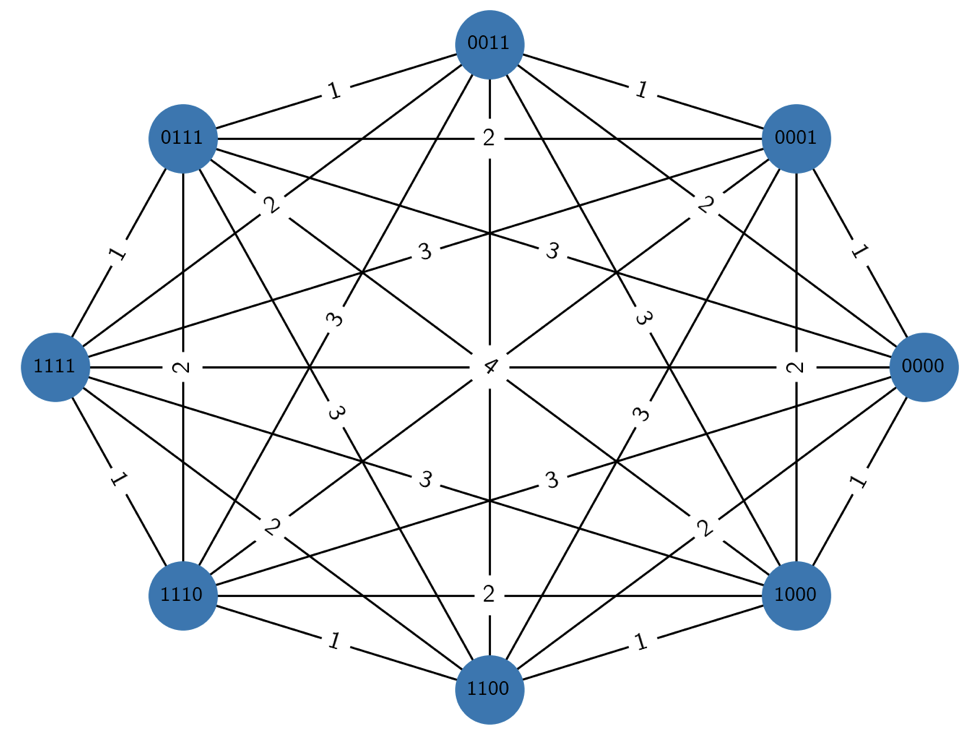
\includegraphics[width=0.6\textwidth]{Images/4qubitreg_graph_bitstrings.png}
    \caption{The graph of the given encoding scheme where the outer ordering of the bit-strings follow the Hamming distance.}
    \label{fig:4q_example_encoding}
\end{figure}

For the 4-qubit encoding scheme, we obtain a fully connected graph as defined by Fig.~\ref{fig:4q_example_encoding}, where again the respective positions of the bit-strings reflect the Hamming distance between them. To effectively map a computationally determined basis to these bit-strings, we use the following procedure:

\begin{itemize}
    \item Given the chosen basis tokens, and their positions in the text, create a graph where each basis token is a single node.
    \item Calculate the distances between all token positions given a pairing of each token with the others ($n*(n-1)/2$ pairings).
    \item For simplicity, choose the minimum distances between each of the pairings, and create edges with this as the given weight. [Note: alternative methods can also be used: mean, median, etc]
    \item With the given fully-connected graph, find a Hamiltonian cycle, and use the returned ordering to map the tokens onto the bit-strings.
\end{itemize}

For any given Hamiltonian cycle, the relationships between each of the tokens will be preserved, and can effectively be mapped onto the bit-string encodings. It can be noted that alternative encoding schemes, and distance orderings could potentially be investigated, but will remain beyond the scope of this current project. Using the above scheme and method, we have determined a given ordering for an 8-basis bit-string set from Lewis Carroll's ``Alice in Wonderland'' as:
\begin{equation}
\begin{array}{cccccc}
\textrm{Alice} & \rightarrow & \vert 0000\rangle, & \textrm{Hatter} & \rightarrow &\vert 0001\rangle, \\
\textrm{King} & \rightarrow & \vert 0011 \rangle, & \textrm{Queen} & \rightarrow &\vert 0111\rangle, \\
\textrm{time} & \rightarrow & \vert 1111 \rangle, &\textrm{Mock} & \rightarrow &\vert 1110\rangle, \\
\textrm{Turtle} & \rightarrow & \vert 1100\rangle, &\textrm{Gryphon} & \rightarrow &\vert 1000\rangle.
\end{array}
\label{eq:aiw_order}
\end{equation}
 with the resulting graph order mapped onto the Fig.~\ref{fig:4q_example_encoding} structure shown by Fig.~\ref{fig:4q_aiw}.

\begin{figure}[htbp]
    \centering
    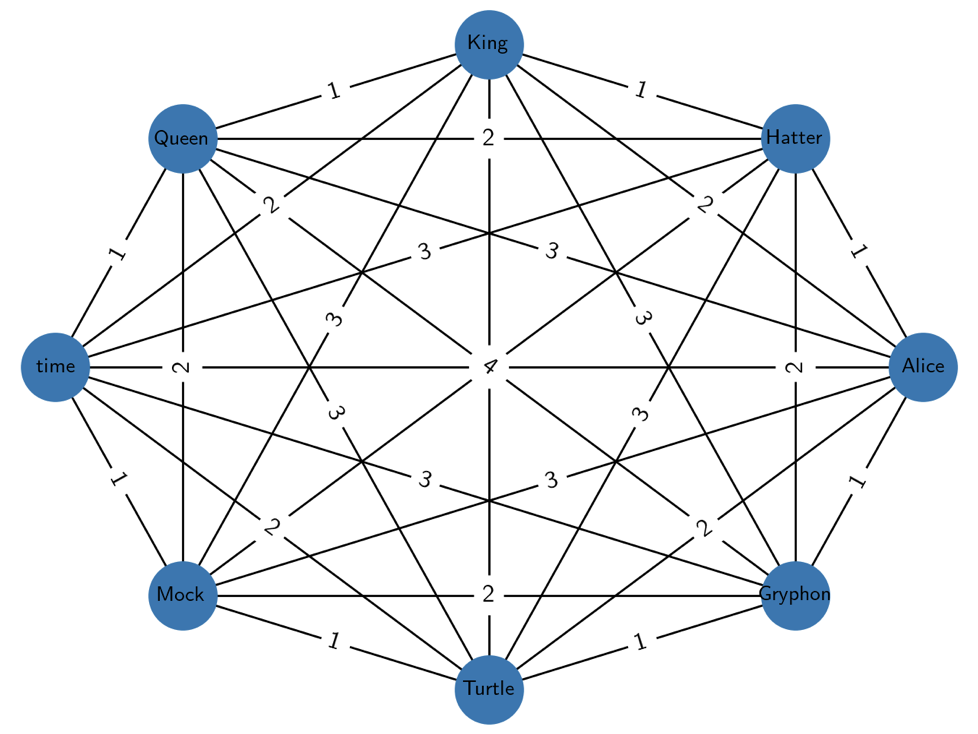
\includegraphics[width=0.6\textwidth]{Images/4qubitreg_graph_aiw.png}
    \caption{Relative ordering of an 8-basis set chosen for the noun dataset in `Alice in Wonderland', using the ordering given by \eqref{eq:aiw_order}.}
    \label{fig:4q_aiw}
\end{figure}

With the above mappings defined, we can now map the composite tokens onto the chosen basis encoding using a distance cut-off. Following the inter-word distance calculation approach used to determine basis order, we determine the distance between the other corpus tokens and the respective basis set, wherein a composite token $c$ is a superposition of a given subset of bases, $b_s$, if each item in the subset is within a given cut-off distance from the composite token position. While other distance metrics may be chosen, for the purpose of clarity and simplicity, this one is used going forward. The mapped composite tokens may then be used to create a compositional sentence structure by tensoring the respective token states. 

An example of this mapping given a different basis set (using alternative distance metrics) is shown in Fig.~\ref{fig:aiw_composite_map}. Here we map the tokens `hall' and `table' to the basis using distances as the metric, and demonstrate the similarity between the tokens by their respective state overlaps. The states themselves are given as 
\begin{equation}
\begin{array}{lll}
\vert \textrm{hall} \rangle &= &a_0\vert \textrm{round} \rangle + a_1\vert \textrm{Rabbit} \rangle + a_2\vert \textrm{head} \rangle \\
 & + &a_3\vert \textrm{way} \rangle + a_4\vert \textrm{time} \rangle + a_5\vert \textrm{Alice} \rangle, \\
\vert \textrm{table} \rangle &= &b_{0}\vert \textrm{March} \rangle  + b_{1}\vert \textrm{tone} \rangle  + b_{2}\vert \textrm{round} \rangle  \\
 & + &b_{3}\vert \textrm{nothing} \rangle  + b_{4}\vert \textrm{Hare} \rangle + b_{5}\vert \textrm{things} \rangle  \\ 
 & + & b_{6}\vert \textrm{thing} \rangle  + b_{7}\vert \textrm{way} \rangle  + b_{8}\vert \textrm{King} \rangle \\ & + &b_{9}\vert \textrm{time} \rangle  + b_{10}\vert \textrm{Alice} \rangle.
\end{array}
\end{equation}

\begin{figure}[htbp]
    \centering
    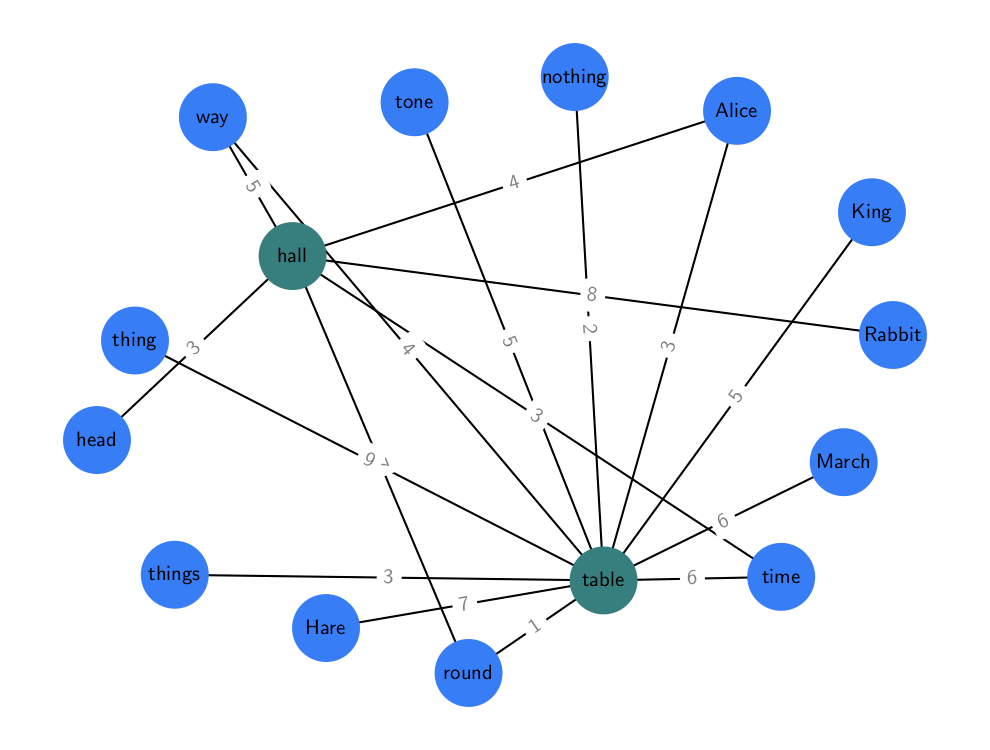
\includegraphics[width=0.6\textwidth]{Images/aiw_composite_mapped.png}
    \caption{Sample mapping of composite tokens (green) to basis tokens (blue) in AIW.}
    \label{fig:aiw_composite_map}
\end{figure}


%---------------------------------------------------------------------------------
%---------------------------------------------------------------------------------
\newpage
\section{MPI}
\label{sec:MPI}
MPI was enabled for the QNLP library allowing for experiments to be scaled across a distributed computing system. 

\subsection{Implementation}
\label{sec:Enabling_MPI__Implmentation}
This was simply done by adding a \textit{MPI\_Comm\_rank} call in the constructor of the \textit{IntelSimulator} class so that each MPI process had it's rank identifier. This was necessary, since in the \textit{applyMeasurement} member function of the \textit{IntelSimulator} class, a random number must be generated and distributed to all processes so that the same random number is being used to randomly collapse a specified qubit across all states in the superposition. If each process had it's own unique random number, this measurement would behave incorrectly, yielding incorrect results.

The Python layer also works using the MPI environment, however \textit{mpi4py} must be imported to set up the MPI environment. During the compilation of the Python bindings, we also compile mpi4py using the given system environment, where mpi4py is subsequently imported during the QNLP library import stage. This allows for the MPI environment to be initialised correctly, and has been verified to operate correctly with the MPI setup on Slurm with ICHEC's Kay supercomputer.

\subsection{Verification}
\label{sec:Enabling_MPI__Verification}
All of the unit tests passed using a distributed resource allocation. This would not be the case if MPI was enabled but not behaving as expected. Thus, the MPI implementation works correctly.

\subsection{Building with MPI Enabled}
\label{sec:Enabling_MPI__Building_with_MPI_Enabled}
Finally, in order to enable the MPI environment when using the QNLP library, both the Intel\textregistered-QS library and the QNLP library must be built with the appropriate version of MPI. Note that if the MPI environment is setup when building the QNLP library with CMake, the \textit{MPI\_FOUND} flag will be automatically set, which is the condition that the MPI environment will be compiled with the MPI environment enabled.

\subsection{Running Application with MPI}
\label{sec:Enabling_MPI__Running_Application_with_MPI}
It is also worth noting that the number of processes on a node is not limited to two. A larger number of processes per node can be specified as long as it is a power of two, and that the overall number of processes is a also a power of two. The identification of this misconception allows for better utilisation of a node's memory and compute resources, and a possible reduction in MPI communication overhead due to the locality of processes on a node. This needs to be verified to ensure that the bandwidth both for intra- and inter-node communication does not become an area of contention for larger scale experiments. On ICHEC's HPC system, Kay, each node is composed of two sockets, each with $20$ physical cores. Due to Intel\textregistered-QS's requirement that the number of processes must be power of two, a maximum of 32 processes can be run on each node.

%---------------------------------------------------------------------------------
%---------------------------------------------------------------------------------
\newpage
\section{Optimisations}
\label{sec:optimisations}
Due to the relatively poor scaling performance and the identification of the current most significant bottlenecks, optimisations are being applied to the QNLP library for the final scaling experiments to be carried out during the last stage of the project. These optimisations mainly consist of algorithmic changes to the decomposition of the $n$-controlled unitary (\textit{NCU}) operations into the fundamental gate-set made available by the underlying quantum simulator. Following the gate-set decomposition procedures discussed in \cite{Barenco_1995}, we can achieve an order or magnitude reduction in gate operations. The scaling of the decomposition for both the default and optimised routines is given by Fig.~\ref{fig:ncu_opt}.


\begin{figure}[!h]
\centering
\begin{tikzpicture}
\begin{axis}[
    title={Decomposition of n-controlled $\sigma_x$ gate to 2-qubit gates},
    xlabel={Number of control lines},
    ylabel={Number of 2-qubit gates},
    xmin=1, xmax=14,
    %ymin=0, ymax=1200,
    xtick={2,4,6,8,10,12},
    ytick={1,10,100, 1000, 10000, 100000,1000000},
    legend pos=north west,
    ymajorgrids=true,
    grid style=dashed,
    ymode=log,
    scale only axis,
    width=0.75\textwidth,
]
\addplot[
    color=blue,
    mark=square,
    ]
    coordinates {
    (2, 5)
    (3, 17)
 (4, 53)
 (5, 161)
 (6, 485)
 (7, 1457)
 (8, 4373)
 (9, 13121)
 (10, 39365)
 (11, 118097)
 (12, 354293)
 (13, 1062881)
    };
\addplot[
    color=red,
    mark=triangle,
    ]
    coordinates {
    (2,5)
(3, 13)
 (4, 41)
 (5, 60)
 (6, 182)
 (7, 146)
 (8, 440)
 (9, 1322)
 (10, 3968)
 (11, 11906)
 (12, 35720)
 (13, 107162)
 };
    \legend{Default, {3,5,7}-CX optimised} 
\end{axis}
\end{tikzpicture}
\caption{The 2-qubit gate operations generated by the n-controlled unitary decomposition. The default method is the current implementation, where the optimised {3,5,7}-method optimises the decompositions where applicable.}
\label{fig:ncu_opt}
\end{figure}

While using the 3,5,7 optimisations still scales exponentially, the offset for larger control operations shows approximately an order of magnitude improvement in number of calls. This will be essential to attempting large-scale runs of the end-to-end implementation during the final stage of the project.


%---------------------------------------------------------------------------------
%---------------------------------------------------------------------------------
\newpage
\section{Application Profiling}
\label{sec:Application_Profiling}
After conducting some initial scaling experiments on the 'closest vector problem' algorithm, it became evident that scalability is an issue. Therefore, it was decided to profile the application in the search for bottlenecks and their causes. The Intel\textregistered Parallel Studio XE performance analysis tool suite was used to profile the application to gain an overview of the performance and inspect any issues in greater detail.

The profiling results shown in this section compare the performance of the application before and after applying optimisations to the \textit{nCU} gate routine discussed in Section~\ref{sec:optimisations}. Note that the \textit{nCU} optimisations did not produce the correct results, but are of a similar type and number of gates as the expected correct implementation. Thus, the comparisons provided in this section are meaningful and represent the expected optimised \textit{nCU} implementation that yields the correct results.

A number of scripts were created to launch and run each profiling tool due to the different environments required for each tool. Note, the profiling with hardware counters enabled on Kay was limited to using a maximum of four nodes since they are the only nodes with the appropriate permissions for hardware counters. A small number of processes was used to reduce the quantity of data collected.

The profiling experiments listed below were carried out using an allocation of $2$ nodes, each with $2$ processes running a single thread. The length of the binary string used was $6$ which corresponds to a quantum register with $14$ qubits. The experiments were run for $1000$ iterations. 

\subsection{Intel\textregistered VTune Application Performance Snapshot (APS)}
\label{sec:Intel_aps}
To get a summary of the current most significant bottleneck, the Intel\textregistered VTUNE Application Performance Snapshot tool was used to conduct an initial profile of the application. A summary of these profiling results can be seen in Figure~\ref{fig:aps}. 

\begin{figure}[H]%[!ht]
    \centering
    \begin{subfigure}{.8\linewidth}
        \centering
        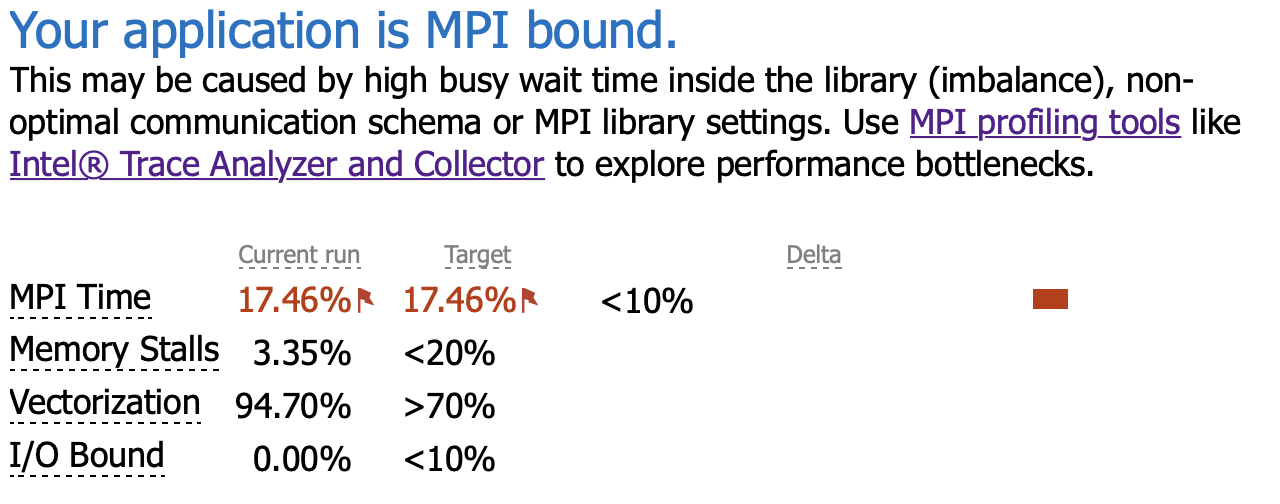
\includegraphics[width=1.\linewidth]{Images/VTUNE_APS/original.png}
		\caption{Unoptimised NCU implementation. Total compute time was $783.33$s.}
        \label{fig:aps_unopt_ncu}
    \end{subfigure}\\
    \begin{subfigure}{.8\linewidth}
        \centering
        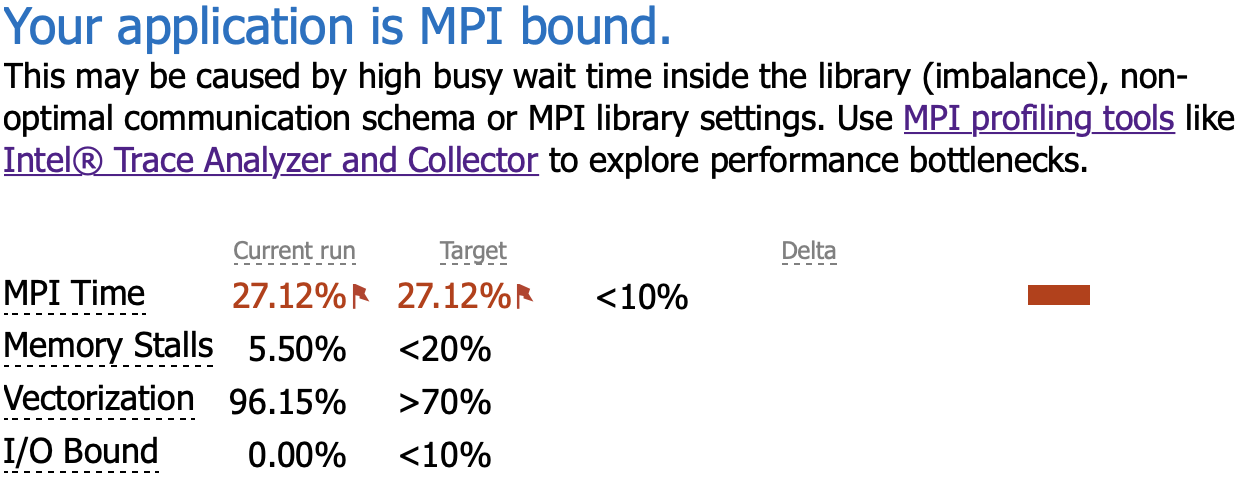
\includegraphics[width=1.\linewidth]{Images/VTUNE_APS/ncu_opt.png}
		\caption{Optimised NCU implementation. Total compute time was $449.91$s.}
        \label{fig:aps_opt_ncu}
    \end{subfigure}
    \caption{APS summaries for both unoptimised and optimised NCU operations for the application. Note, the reduction in the runtime of the the optimised routine in Figure~\ref{fig:aps_opt_ncu}.}
        \label{fig:aps}
\end{figure}

In both cases, it reported that the application is MPI bound and recommended a more detailed profiling analysis using the Intel\textregistered Trace Analyzer \& Collector.

Although the percentage of time spent in MPI routines increased after applying the optimisation, the runtime has almost halved. The time spent in vectorised routines increases. To gain a better understanding of the behaviour, further profiling was conducted.


\subsection{Intel\textregistered Trace Analyzer \& Collector (ITAC)}
\label{sec:Intel_ITAC}
Upon the recommendation of the the Intel\textregistered VTune APS, the ITAC tool was run for both versions of the application. It collects and analyses the inter-process communication including between nodes. 

\subsubsection{Serial versus Parallel Comparison}
Figure~\ref{fig:itac_pie} shows the percentage of total run-time spent in serial, MPI, and threaded regions. The percentage of time spent on serial regions decreases by $1.2\%$, but MPI regions increase by $6.2\%$ after the \textit{nCU} optimisations. 

\begin{figure}[H]%[!ht]
    \centering
    \begin{subfigure}{1.\linewidth}
        \centering
        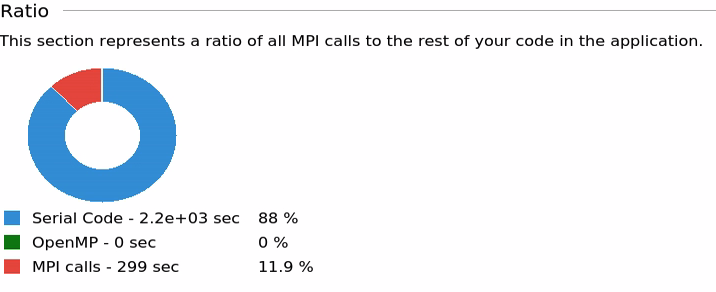
\includegraphics[width=1.\linewidth]{Images/MPI_Serial_Pie/orig_pie.png}
		\caption{Unoptimised NCU implementation.}
        \label{fig:itac_pie_unopt_ncu}
    \end{subfigure}\\
    \begin{subfigure}{1.\linewidth}
        \centering
        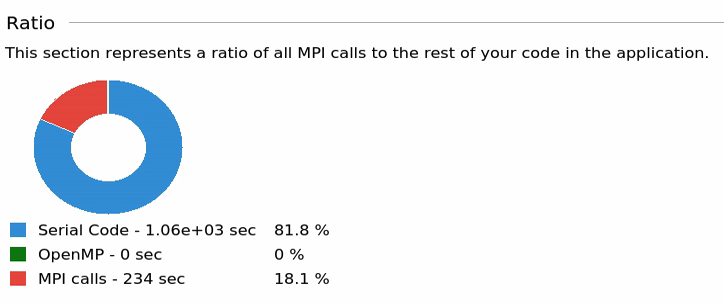
\includegraphics[width=1.\linewidth]{Images/MPI_Serial_Pie/ncu_pie.png}
		\caption{Optimised NCU implementation.}
        \label{fig:itac_pie_opt_ncu}
    \end{subfigure}
    \caption{ITAC breakdown of time spent in serial, MPI and OpenMP sections     for both unoptimised and optimised NCU operations for the application.}
        \label{fig:itac_pie}
\end{figure}

Taking the significant reduction in runtime by almost $50\%$ into account after the optimisations, it is clear that the time spent in both MPI and serial regions have decreased significantly. Now MPI routines are taking up a larger percentage of the runtime.

\subsubsection{Overview of MPI Routines}
\label{sec:overview_MPI_routines}
The breakdown of the comparison between each of the most active MPI routines are visible in Figure~\ref{fig:itac_mpi_bar}. \textit{MPI\_Sendrecv} is responsible for the majority of MPI overhead. \textit{MPI\_Comm\_size} and \textit{MPI\_Comm\_rank} respectively contribute a lot less but still relatively significantly to the MPI overhead. This did not change after the \textit{nCU} optimisations were applied. The runtime for each of these routines decreased but their percentage contribution to the runtime increased.

\begin{figure}[!ht]
    \centering
    \begin{subfigure}{1.\linewidth}
        \centering
        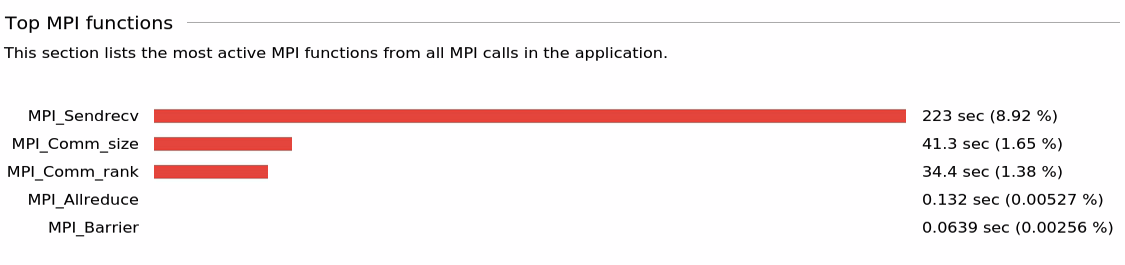
\includegraphics[width=1.\linewidth]{Images/MPI_Comms_Bar/orig_comms_bar.png}
		\caption{Unoptimised NCU implementation.}
        \label{fig:itac_mpi_bar_unopt_ncu}
    \end{subfigure}\\
    \begin{subfigure}{1.\linewidth}
        \centering
        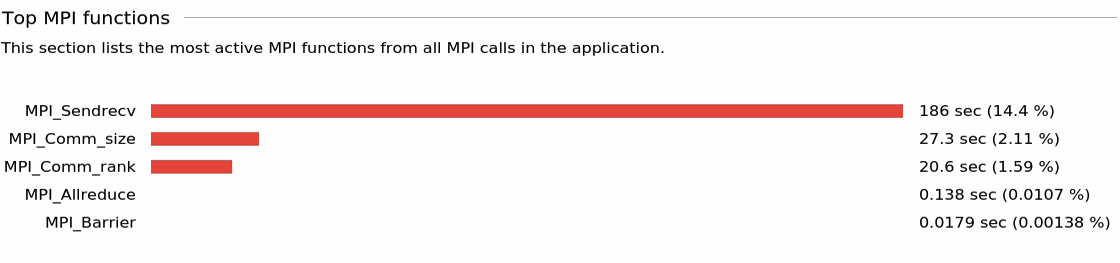
\includegraphics[width=1.\linewidth]{Images/MPI_Comms_Bar/ncu_comms_bar.png}
		\caption{Optimised NCU implementation.}
        \label{fig:itac_mpi_bar_opt_ncu}
    \end{subfigure}
    \caption{ITAC summary breakdown of time spent in different MPI routines for both unoptimised and optimised NCU operations for the application.}
        \label{fig:itac_mpi_bar}
\end{figure}

\subsubsection{Event and Quantitative Timelines}
An event timeline and quantitative timeline can be seen in Figure~\ref{fig:itac_comms_bar} for approximately a single iteration of both the unoptimised and optimised versions of the application. First, note that Figure~\ref{fig:itac_mpi_comms_unopt_ncu} is not shown in as fine time resolution as Figure~\ref{fig:itac_mpi_comms_opt_ncu}, so they are not directly quantitatively comparable. The event timeline depicts the MPI communication between each of the four processes. The quantitative timeline more clearly depicts which processes where involved in the communications and the duration of the communications. 

In Figure~\ref{fig:itac_mpi_comms_unopt_ncu}, majority of the MPI communications are across all of the processes. In contrast, in Figure~\ref{fig:itac_mpi_comms_opt_ncu} the MPI communication is rarely across all processes, instead using point-to-point communications. Comparing these two figures, the optimised \textit{nCU} version has in general less expensive MPI communication routines across all of the processes, and thus there is less MPI overhead.

\begin{figure}[H]%[!ht]
    \centering
    \begin{subfigure}{1.\linewidth}
        \centering
        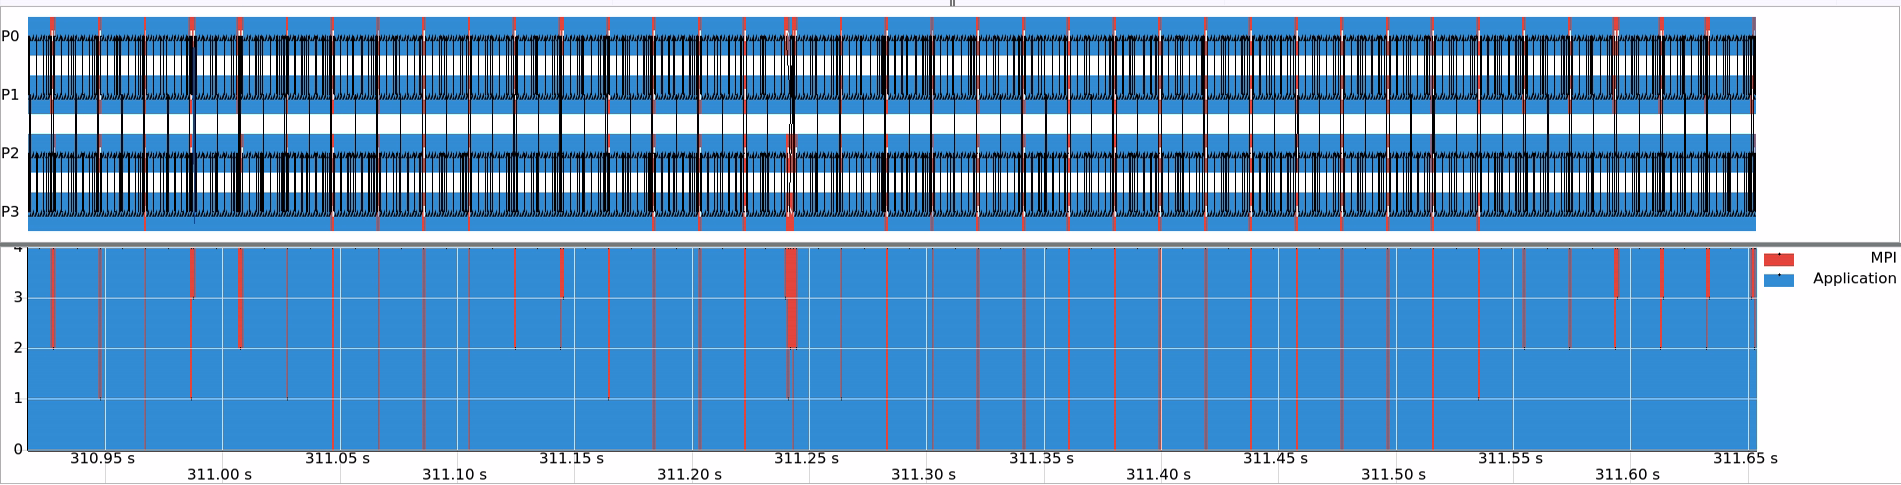
\includegraphics[width=1.\linewidth]{Images/App_iteration/orig_single_iteration.png}
		\caption{Unoptimised NCU implementation.}
        \label{fig:itac_mpi_comms_unopt_ncu}
    \end{subfigure}\\
    \begin{subfigure}{1.\linewidth}
        \centering
        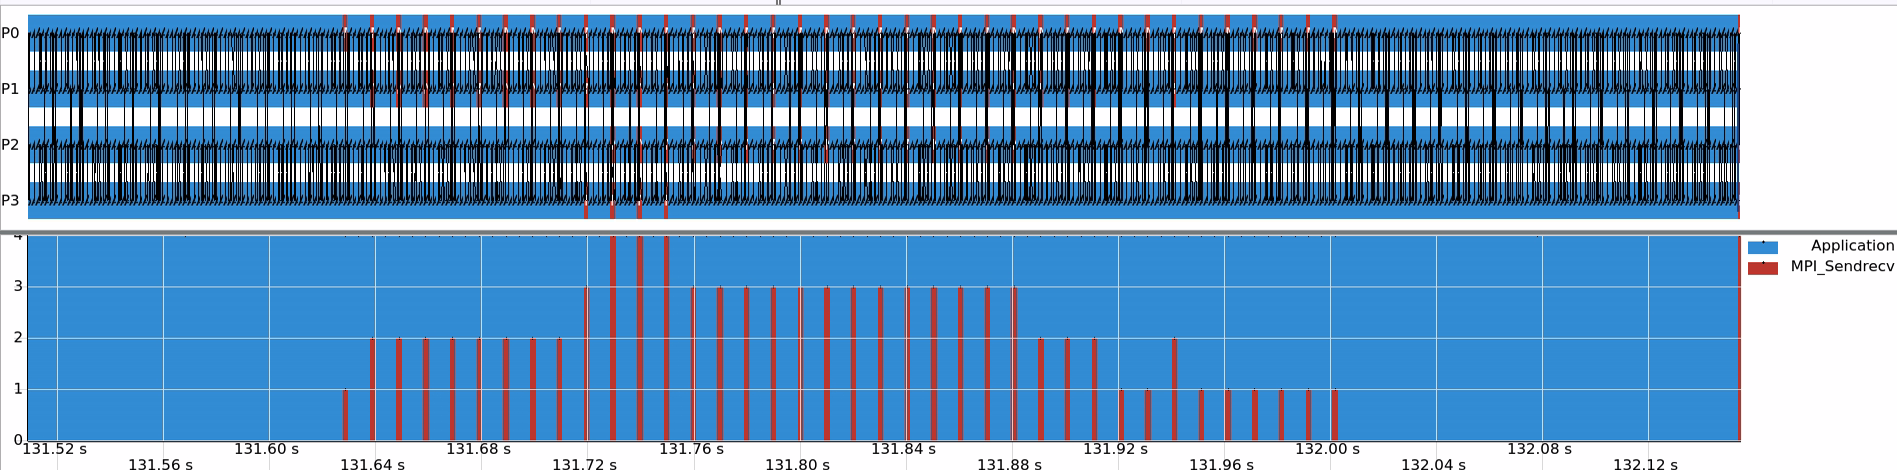
\includegraphics[width=1.\linewidth]{Images/App_iteration/ncu_single_iteration.png}
		\caption{Optimised NCU implementation.}
        \label{fig:itac_mpi_comms_opt_ncu}
    \end{subfigure}
    \caption{ITAC event (top of each subfigure) and quantitative (bottom of each subfigure) timelines for approximately a single iteration of both the unoptimised and optimised \textit{nCU} operations for the application.}
        \label{fig:itac_comms_bar}
\end{figure}

\subsubsection{MPI Call Counts}
Figure~\ref{fig:itac_counts_unopt_ncu} and~\ref{fig:itac_counts_opt_ncu} detail the call counts and corresponding execution times for the unoptimised and optimised \textit{nCU} routines respectively. The lists are ordered by decreasing call counts. \textit{MPI\_Comm\_size} is called approximately $278\times10^6$ times and $190\times10^6$ for the unoptimised and optimised routines respectively. Similarly, $142\times10^6$ and $98\times10^6$ for \textit{MPI\_Comm\_rank}, $12\times10^6$ and $13\times10^6$ for \textit{MPI\_Sendrecv}, $14\times10^3$ and $2\times10^3$ for \textit{MPI\_Barrier}, and $12\times10^3$ and $0$ for \textit{MPI\_Bcast}. All of the other call counts remained approximately the same.

From Section~\ref{sec:overview_MPI_routines}, \textit{MPI\_Comm\_size} consists of $1-2\%$ of runtime, and \textit{MPI\_Comm\_rank} $1.3-1.6\%$. From Figure~\ref{fig:itac_counts}, they are responsible for a very large number of MPI calls, being called more than any other MPI routine. After applying the \textit{nCU} optimisations, their call counts are reduced considerably, but still account for majority of MPI calls. These two routines should ideally only be called at the very beginning of the application when the MPI environment is initialised. However, Intel\textregistered-QS calls them in its quantum gate calls. Thus, if Intel\textregistered-QS has these calls removed  from its gate calls and instead stores these calls' initial values as constant values, a small but significant overhead will disappear. Also note, these calls only increase as the problem size increases, scaling with the gate depth and hence problem size.

The number of \textit{MPI\_Send\_recv} calls increased by approximately $1\times10^6$ after the optimisations. However, the number of \textit{MPI\_Bcast} was reduced from $12\times10^6$ to zero. The extra \textit{MPI\_Send\_recv} was due to the re-implementation of the \textit{nCU} routine, which also got rid of the need of \textit{MPI\_Bcast}'s. The latter of the two can be considered to be more expensive since it is a group communication rather than just involving two processes (also taking the quantity of the reduction into account), even though \textit{MPI\_Send\_recv} is blocking and \textit{MPI\_Bcast} is not. This explains a portion of the performance increase.

There is also a significant reduction in the number of expensive \textit{MPI\_Barrier} calls after the optimisations. This is a significant improvement.

\begin{figure}[H]%[!ht]
    \centering
    \begin{subfigure}{1.\linewidth}
        \centering
        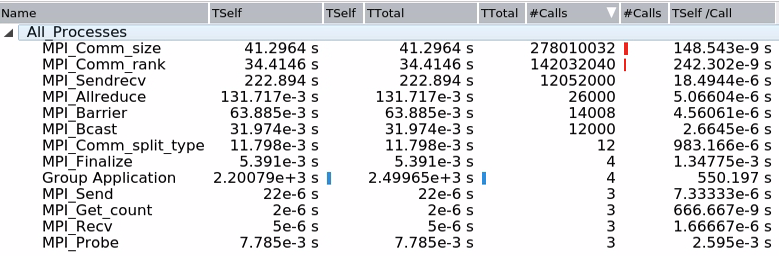
\includegraphics[width=1.\linewidth]{Images/MPI_message_counts/orig_message_counts.png}
		\caption{Unoptimised NCU implementation.}
        \label{fig:itac_counts_unopt_ncu}
    \end{subfigure}\\
    \begin{subfigure}{1.\linewidth}
        \centering
        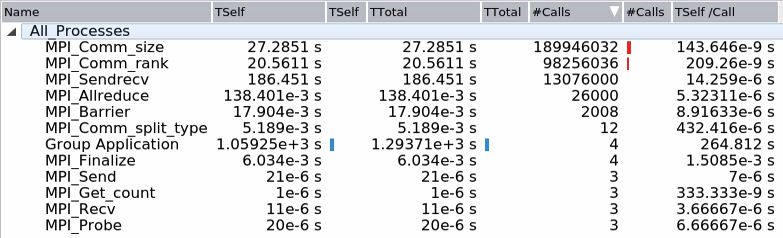
\includegraphics[width=1.\linewidth]{Images/MPI_message_counts/ncu_message_counts.png}
		\caption{Optimised NCU implementation.}
        \label{fig:itac_counts_opt_ncu}
    \end{subfigure}
    \caption{ITAC MPI message counts for both the unoptimised and optimised NCU operations for the application.}
        \label{fig:itac_counts}
\end{figure}

\subsection{Intel\textregistered VTUNE Amplifier}
Intel\textregistered VTUNE Amplifier was used to profile the behaviour of the application on a single node, taking more detailed measurements into consideration including hardware metrics. This allows for a more detailed analysis of the applications behaviour and can indicate individual functions and regions of code that contribute to overhead.

A summary of which source files contribute to the majority of CPU utilisation occurred is shown in Figure~\ref{fig:vtume_amplxe_summary}. The first seven of these source files are from the Intel\textregistered-QS. The first three of these account for the majority of CPU utilization. The biggest contributor is the \textit{highperfkernel.cpp} source file. Upon switching to a view which was grouped by the function call stack, the same observations were made.

The \textit{apply\_ctrl2qubitgate.cpp} source file and the \textit{ncu.hpp} header file were identified as the biggest contributors from the QNLP library. The first of these calls routines from the Intel\textregistered-QS library directly, so cannot be optimised further. Further optimisations are possible for the \textit{nCU} implementation, however due to time constraints, will be put on hold.

\begin{figure}[H]%[!ht]
    \centering
    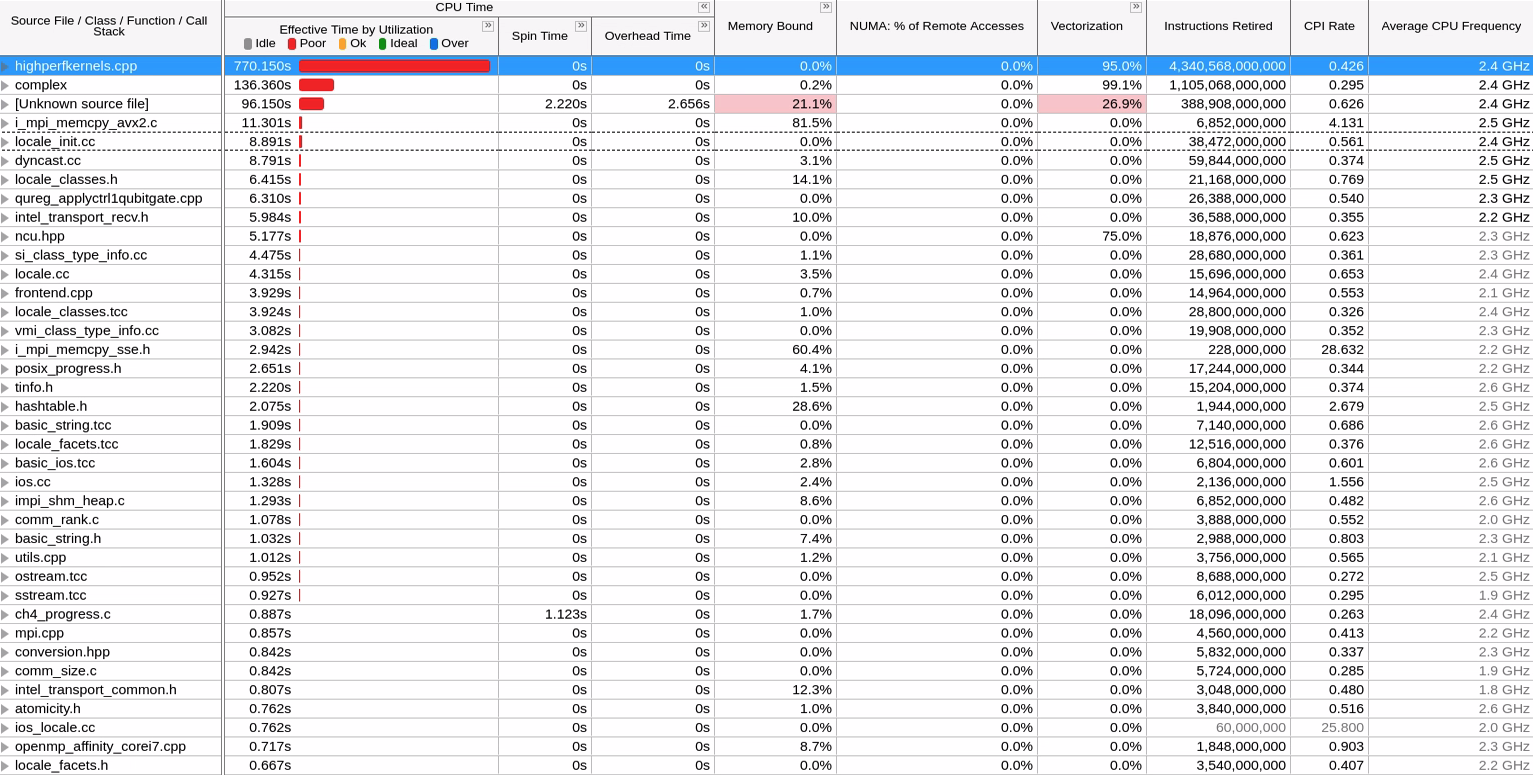
\includegraphics[width=1.\linewidth]{Images/VTUNE_Amplxe/vtune_amplxe_summary.png}
	\caption{Summary of main contributors of CPU utilization using Intel\textregistered VTUNE Amplifier.}
    \label{fig:vtume_amplxe_summary}
\end{figure}

\subsection{Profiling Conclusions}

The increase in the percentage of the MPI routines after the \textit{nCU} optimisations were applied is an expected outcome. The optimisations reduced the amount of quantum gate calls significantly, including multi-qubit controlled gates. This led to less MPI communications being executed, and also to less regions of serial code being executed. However, the other serial parts of the application remained unaffected by these optimisations, thus the percentage of time spent in MPI routines increased despite the runtime decreasing.

The main bottleneck originated from the \textit{nCU} gate calls. The underlying simulator only has a number of more fundamental gate operations available, consisting of single qubit, and one and two qubit controlled gate operations. The \textit{nCU} gate is an $n$ qubit controlled unitary operation. To implement it, it is decomposed into a series of the fundamental operations previously mentioned. These operations often involve MPI communication to execute successfully. As $n$ becomes larger, the number of gate operations that comprise the \textit{nCU} gate call grows very quickly. This \textit{nCU} gate call is used a number of times in the encoding steps of the algorithm. Thus, one of the reasons for the MPI bound nature of the application is apparent. After applying the optimisations, this routine is still a major contributor to the application's overhead. This is because although the circuit depth has been significantly decreased by the optimisations, it is still very large.

Removing the \textit{MPI\_Comm\_size} and \textit{MPI\_Comm\_rank} calls from the gate operations in the Intel\textregistered-QS would give the application (and similar applications) a small but consistent performance increase.

After using the Intel{\textregistered}VTUNE Amplifier, it is evident that the \textit{highperfkernel.cpp} source file from the Intel\textregistered-QS is the biggest contributor to the overhead caused by poor CPU utilization. It would require further and more detailed profiling analysis to identify whether any performance gain can be made, or if it is already optimal. However, making changes to the Intel\textregistered-QS is beyond the scope of this project.

It is noted that further optimisations could be made to the \textit{nCU} implementation which would give a slight performance improvement by reducing the number of gate calls. If time permits, this will be looked into in further detail.


%---------------------------------------------------------------------------------
%---------------------------------------------------------------------------------
\newpage
\section{Scaling of the Application}
\label{sec:Scaling_of_the_Application}
 Experiments were designed to test the scalability of the application. As mentioned in Section~\ref{sec:intro_scaling}, the application did not scale particularly well. Strong scaling experiments were conducted on both single node and multi-node hardware configurations.


\subsection{Experiment Set-up}
Scaling experiments were performed for the 'closest vector problem' using the C++ layer of the QNLP library. This involved encoding a set of binary vectors into a superposition of quantum states, adjusting the amplitude of each state proportionally to the Hamming distance between each state's binary vector and a test vector, followed by a measurement of the state. This was repeated a large number of times to generate a distribution of the measured states. The execution time for this experiment was measured using timing instrumentation. Strong scaling experiments were conducted by varying the number of processes used (compute resources) while maintaining a fixed total problem size (length of binary vector). Weak scaling experiments were not performed due to time constraints, but will be rigorously tested during the next phase of the project. Each individual experiment was run for $500$ iterations.

The reason that the pre-computation steps (involving the parsing of the corpus, tagging, and application of the distributed and compositional semantic algorithms) was not included in these scaling experiments was because they do not directly interact with the quantum simulator. It would be very difficult to find different corpus which would have a problem size that could be proportionally varied for the required range of compute resources needed for the scaling experiments. Furthermore, the pre-computation stage contributes to a relatively very small proportion of the total compute time of the application, and it's output is precisely the binary vectors that are being encoded into the superposition of states, thus the pre-computation can be ignored at this stage of the scaling experiments. If the run-time of the 'closest vector problem' implementation improves significantly, adding the pre-computation steps to the scaling performance analysis will be considered.

The ICHEC HPC cluster Kay was used for all experiments. Each compute node consists of $2\times 20$-core $2.4$ GHz Intel Xeon Gold $6148$ (Skylake) processors, $192$ GiB of RAM, a $400$ GiB local SSD for scratch space and a $100$ Gbit OmniPath network adaptor. This partition has a total of $336$ nodes consisting of $13440$ cores and $63$ TiB of distributed memory.

\subsection{Single Node Scaling}
\label{sec:single_node_scaling}
Scaling experiments were performed on a single compute node with $2^n$ processes for $n=0,1,2,3,4,5$ ($2^5 = 32$ which is the maximum power of $2$ that is below 40, the number of CPU's on a node, which is a constraint of the Intel\textregistered-QS). Strong scaling was conducted using a binary string length of 6 which implies a total of $2\times 6 + 2 = 14$ qubits were used during the computation. The plotted results of these experiments are shown in Figure~\ref{fig:scaling_single_node}. The full table of results are shown in Table~\ref{tab:scaling_results}.

From observing Figure~\ref{fig:scaling_single_node}, the application achieves near linear scaling for a smaller number of processes which begins to diverge as the number of processes increases. This is an expected result. Also, note that for a single process the execution time is $1903$ seconds, which decreases by an order of magnitude for $8$ or more processes. Thus, the application scales well on a single node for a relatively small problem size and increasing the number of processes has a significant effect on reducing the execution time.


\begin{figure}[htbp]
    \centering
    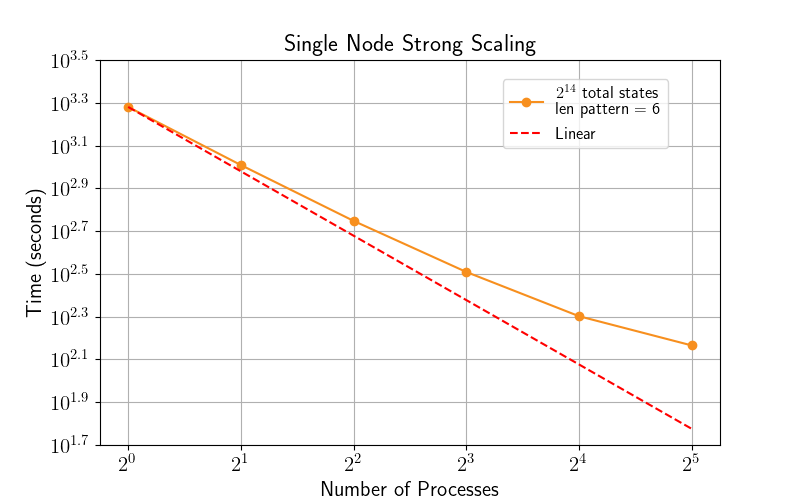
\includegraphics[width=0.95\textwidth]{Images/Scaling/Single_Node_Strong_binlen6.png}
    \caption{Scaling of the application for varying number of processes on a single node, each with one thread. The length of the binary string was $6$ which means a total of $14$ qubits were used. The linear scaling plot is shown in red.}
    \label{fig:scaling_single_node}
\end{figure}

\subsection{Multi-Node Scaling}
\label{sec:multi_node_scaling}
Scaling experiments were also performed for a varying number of processes per node on varying numbers of nodes. This was done to see the effect of MPI communication overhead across nodes as the number of nodes and subsequently processes were increased.

A single strong scaling experiment was conducted by fixing the number of processes per node and the problem size. The total number of processes was then increased by increasing the number of nodes used. This experiment was repeated for varying numbers of processes per node. The problem size was fixed, using a binary string length of $8$, which means the total number of qubits used was $2\times 8 + 2 = 18$. The number of nodes used was $1,2,4,8,16$ and $32$, each with $8,16$ and $32$ processes per node. The plotted results of these experiments are shown in Figure~\ref{fig:scaling_multi_node}. The complete list of results are shown in Table~\ref{tab:scaling_results}.

From observing Figure~\ref{fig:scaling_multi_node}, the application scales almost identically as the number of processes is increased but on different numbers of nodes (different numbers of processes per node). This indicates that inter-node MPI communication does not have a significant impact on the application's scaling for small to medium problem sizes. However, this will need to be tested for larger problem sizes that saturate a node's memory to fully determine. This is because for an experiment, each quantum state can fit in the cache simultaneously. 

The linear scaling for $8$ processes per node is shown in red. Comparing the scaling of each experiment to the linear scaling, the application scales almost linearly for smaller numbers of processes per node, but diverges as the number of processes increases. This is consistent with the observed results for a single node in Section~\ref{sec:single_node_scaling}. Note, for $32$ processes and greater, the execution time is at least an order of magnitude smaller than for $8$ processes. Thus, increasing the number of processes has a significant effect on reducing the execution time.

\begin{figure}[htbp]
    \centering
    \includegraphics[width=0.95\textwidth]{Images/Scaling/multi_node_scalingstrong.pdf}
    \caption{Scaling of the application for varying number of processes on multiple nodes, each with one thread. Every experiment had a fixed number of processes per node. The length of the binary string was $8$ which means a total of $18$ qubits were used. The linear scaling for $8$ processes per node is also shown in red.}
    \label{fig:scaling_multi_node}
\end{figure}

\subsection{Scaling Results}
Table~\ref{tab:scaling_results} details the results of all the scaling experiments conducted for this deliverable. The findings of these results have already been detailed in Sections~\ref{sec:single_node_scaling} and~\ref{sec:multi_node_scaling}. One further point to note about these results is the memory usage per node for the given problem sizes. The largest amount of memory used on a node was $2$MB in these experiments. This was for a binary length of $8$ on a single node. The available memory per node is $192$GB. Thus, the memory usage per node is under-utilised. However, as the number of qubits increases, the number of gate calls in the \textit{nCU} operation explodes, thus increasing the run-time significantly. This was tested for the experiments listed in Table~\ref{tab:scaling_results} using a binary length of $9$ (20 qubits), however these experiments scaled very poorly. Thus, for larger problem sizes, the application does not scale well. Further scaling experiments for larger problem sizes need to be conducted to observe the application's behaviour better. However, these will be conducted on the optimised \textit{nCU} implementation of the application which is expected to scale much better than the current version. The optimised version of the application is still expected to not scale too well due to the large number of gate calls that remain in the \textit{nCU} decomposition.

\begin{table}[h!]
\centering
    \begin{tabular}{||c|c|c|c|c|c|c|c||}
        \hline
        Nodes    &  Procs  &    Num   & Bin       &    Storage &    StoragePer   &    StoragePerNode    &    Time    \\
             &   PerNode  &   Procs    &   Len        &    PerNode  &    State     &    Temporary     &       \\
            &      &       &           &     (MB) &     (MB)    &     (MB)    &  (s)     \\         
        \hline
        \hline
         1   &   1   &   1   &   6   &     0.38    &   0.25    &   0.12500 &   1903    \\
         1   &   2   &   2   &   6   &     0.38    &   0.25    &   0.12500 &   1018    \\
         1   &   4   &   4   &   6   &     0.38    &   0.25    &   0.12500 &   558 \\
         1   &   8   &   8   &   6   &     0.38    &   0.25    &   0.12500 &   322 \\
         1   &   16  &   16  &   6   &     0.38    &   0.25    &   0.12500 &   200 \\
         1   &   32  &   32  &   6   &     0.38    &   0.25    &   0.12500 &   146 \\
         \hline
         1   &   32  &   32  &   8   &     6.00    &   4.00    &   2.00000 &   34856   \\
         2   &   32  &   64  &   8   &     3.00    &   2.00    &   1.00000 &   18852   \\
         4   &   32  &   128 &   8   &     1.50    &   1.00    &   0.50000 &   10868   \\
         8   &   32  &   256 &   8   &     0.75    &   0.50    &   0.25000 &   6663    \\
         16  &   32  &   512 &   8   &     0.38    &   0.25    &   0.12500 &   4562    \\
         32  &   32  &   1024    &   8   &     0.19    &   0.12    &   0.06250 &   3618    \\
         \hline
         1   &   16  &   16  &   8   &     6.00    &   4.00    &   2.00000 &   67360   \\
         2   &   16  &   32  &   8   &     3.00    &   2.00    &   1.00000 &   35058   \\
         4   &   16  &   64  &   8   &     1.50    &   1.00    &   0.50000 &   19022   \\
         8   &   16  &   128 &   8   &     0.75    &   0.50    &   0.25000 &   11020   \\
         16  &   16  &   256 &   8   &     0.38    &   0.25    &   0.12500 &   6624    \\
         32  &   16  &   512 &   8   &     0.19    &   0.12    &   0.06250 &   4743    \\
         \hline
         1   &   8   &   8   &   8   &     6.00    &   4.00    &   2.00000 &   131896  \\
         2   &   8   &   16  &   8   &     3.00    &   2.00    &   1.00000 &   67604   \\
         4   &   8   &   32  &   8   &     1.50    &   1.00    &   0.50000 &   35216   \\
         8   &   8   &   64  &   8   &     0.75    &   0.50    &   0.25000 &   19080   \\
         16  &   8   &   128 &   8   &     0.38    &   0.25    &   0.12500 &   10981   \\
         32  &   8   &   256 &   8   &     0.19    &   0.12    &   0.06250 &   6721    \\
        \hline
        \hline
    \end{tabular}
    \caption{Results of all scaling experiments shown in plots. Each individual experiment was run for $500$ iterations.}
    \label{tab:scaling_results}  
\end{table}




%---------------------------------------------------------------------------------
%---------------------------------------------------------------------------------
\newpage
\section{Discussions and Summary}
\label{sec:discussion_and_summary}

In this document we have discussed the complete workflow of the application including the Python bindings of the C++ layer which allows for the execution of the entire application in Python. A new basis word encoding strategy that takes the relative differences in the meanings of the basis words into account for the encoding was introduced and has been implemented. The QNLP library and by extension the application has now been successfully implemented with MPI enabled which allows for scaling of the application to larger problem sizes. MPI can also be used for the application's Python workflow which uses mpi4py to setup the environment which is then used in the C++ back-end. Optimisations have been implemented to the \textit{nCU} routine which decrease the number of gate calls by an order of magnitude, thus significantly increasing the performance. This optimisation is still in progress, but it almost complete. The application was profiled, identifying bottleknecks in the application and the Intel\textregistered-QS. As discussed, the \textit{nCU} bottleneck is being addressed, however the bottlenecks due to the Intel\textregistered-QS are beyond the scope of this project. Finally, strong scaling experiments were conducted for the application. It was observed that it is worth utilising the maximum allowed processes per node to increase performance. Thus, $32$ processes per node should be used. There is no significant MPI overhead between nodes that does not exist on a single node for relatively small problem sizes. The application was observed to scale quite well for small problem sizes, however scaling quickly becomes a significant issue as the problem size increases. Further scaling experiments will be conducted for the optimised \textit{nCU} implementation of the application.

%---------------------------------------------------------------------------------
%---------------------------------------------------------------------------------
%\newpage
%\begin{appendices}

\end{appendices}




%---------------------------------------------------------------------------------
\newpage
%---------------------------------------------------------------------------------
%---------------------------------------------------------------------------------
%\bibliographystyle{plain}
\bibliographystyle{unsrt}
\bibliography{Bibliography.bib}

\end{document}
